\section{Introduction}

The use of neural networks as a tool in condensed matter research has seen a growth in popularity. One of the marvels and advantages of this technique is how little statistical-physics information (energies, order parameters, etc.) is needed for the classification of states or the pinpointing of critical physical parameters.
Even relatively simple neural network models can learn phase-transition temperatures, order parameters, and quantum-state tomography, from the information of a simple feature such as position coordinates in an off-lattice model or the location and value of spins in an Ising model. This could all be done without any knowledge of the original Hamiltonian or interaction potential energies \cite{torlaiboltzmann,carras,wei,wetzel,torlai,morningstar,beach}.


\begin{figure*}[!t]
	\centering
	\begin{minipage}[t]{0.25\textwidth}
		\centering
		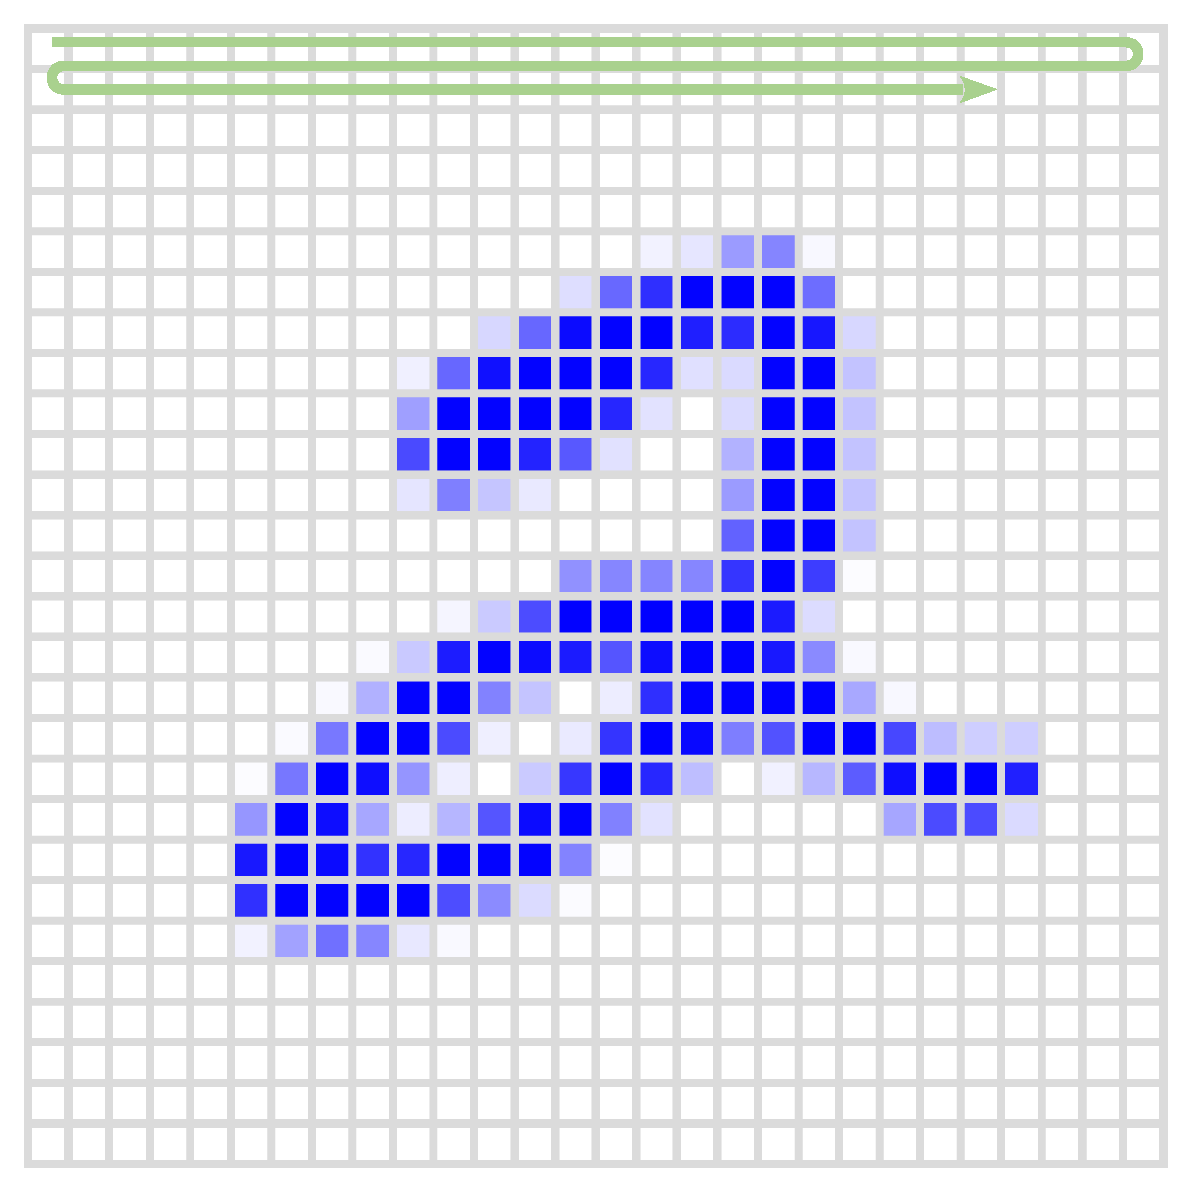
\includegraphics[width=0.9\columnwidth]{./figs/FIG1A.eps}\\
		(a)\\ \vspace{0.5cm}
		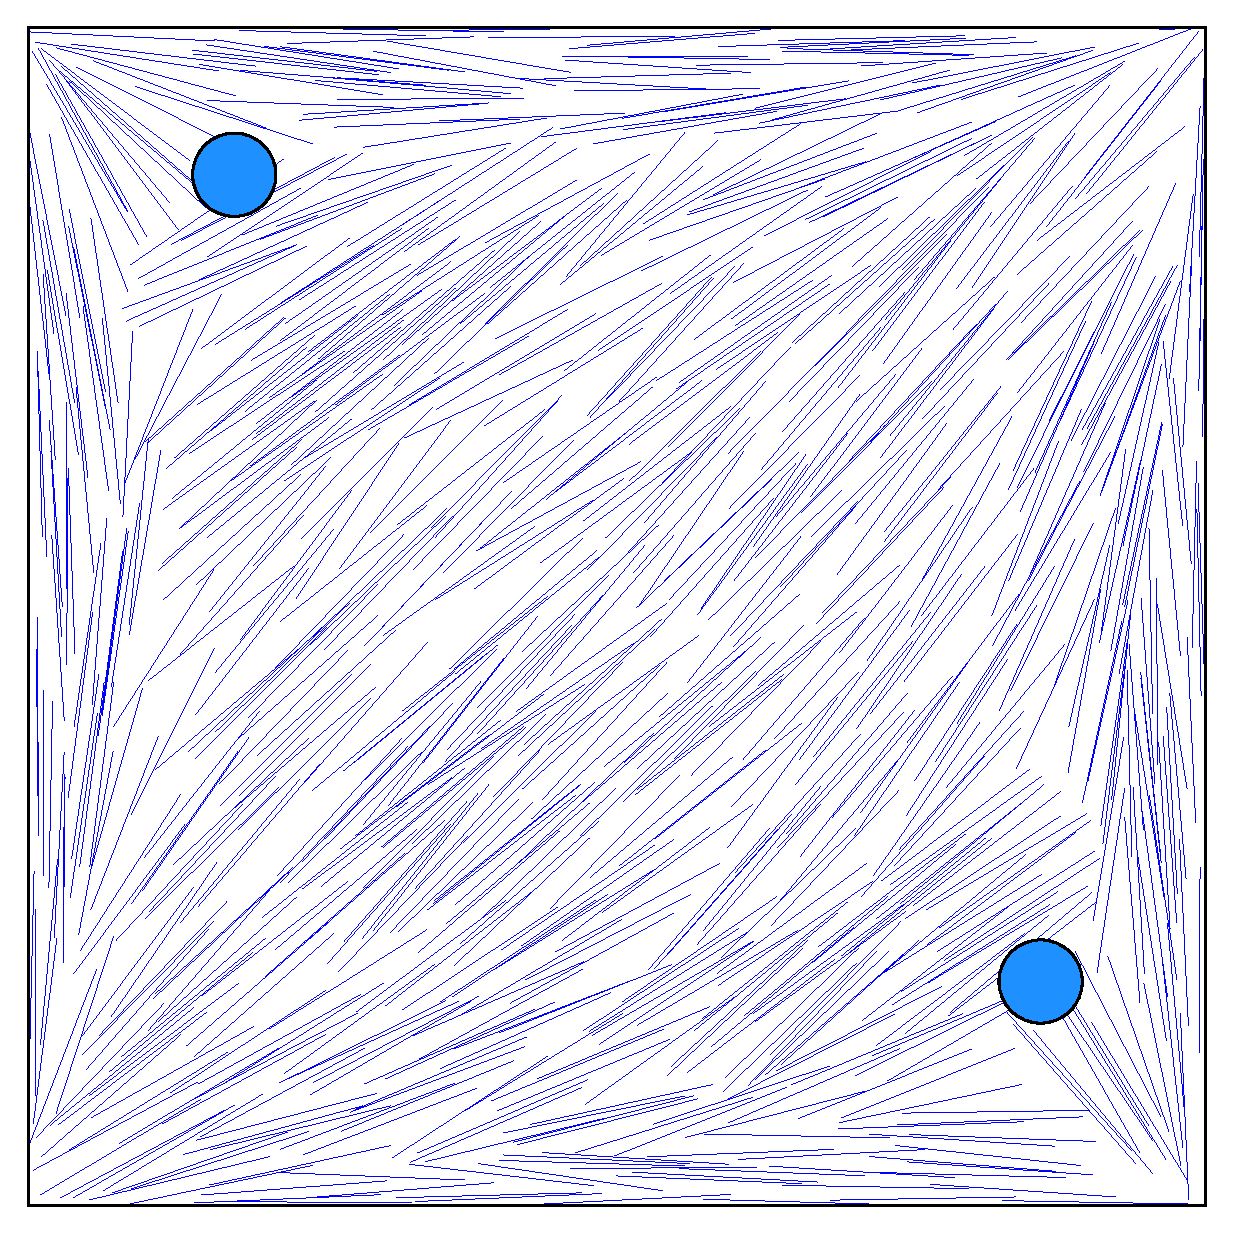
\includegraphics[width=0.9\columnwidth]{./figs/FIG1E.eps}\\
		(e)
	\end{minipage}%
	\begin{minipage}[t]{0.25\textwidth}
		\centering
		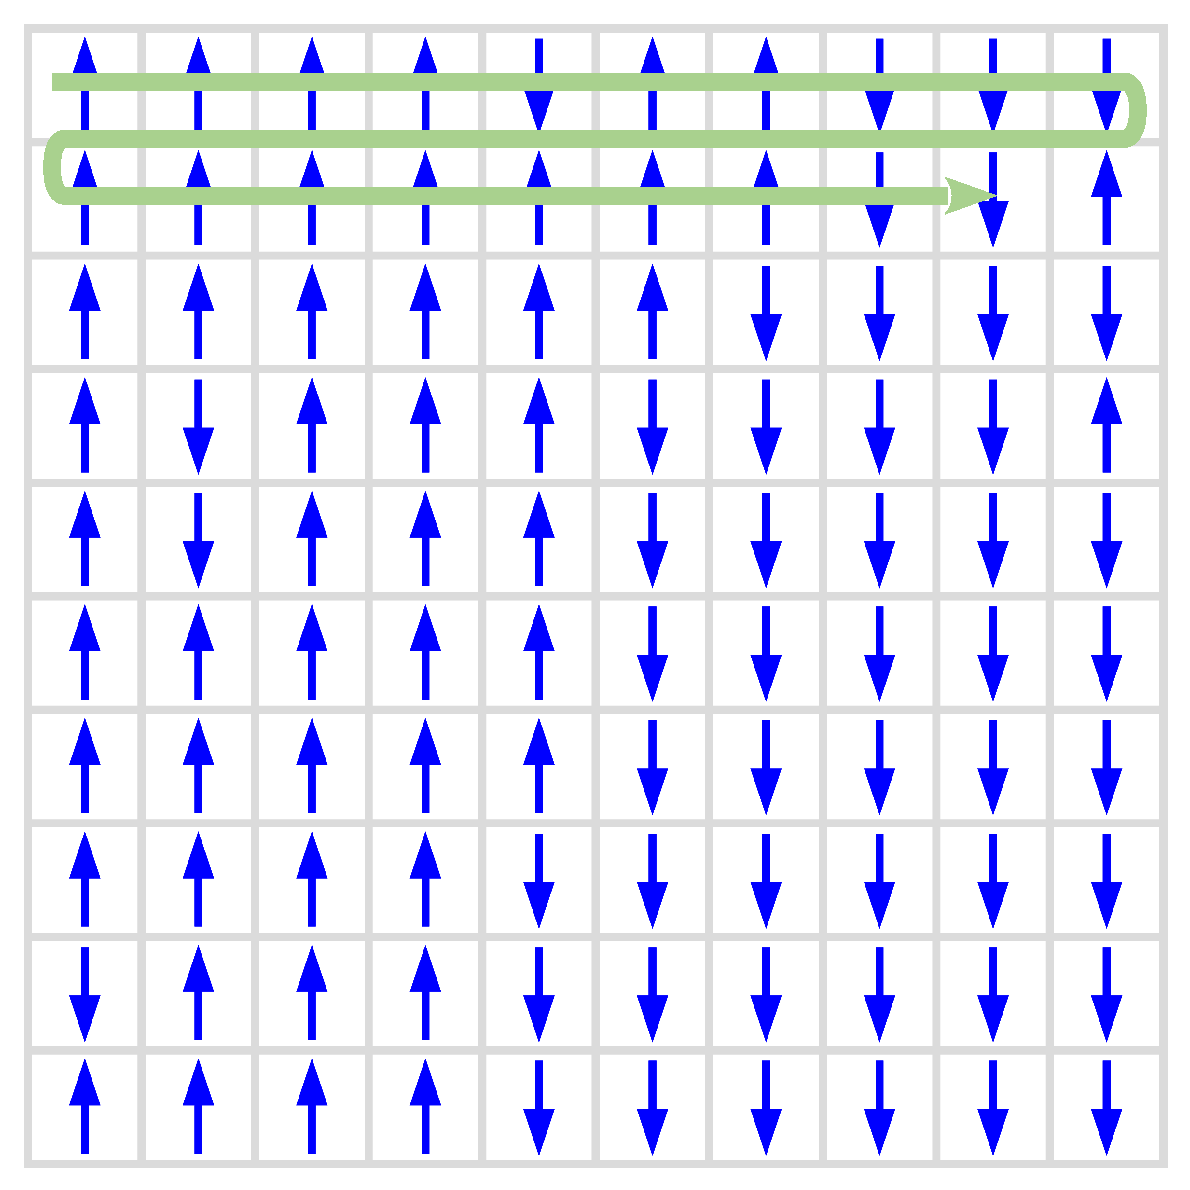
\includegraphics[width=0.9\columnwidth]{./figs/FIG1B.eps}\\
		(b)\\ \vspace{0.5cm}
		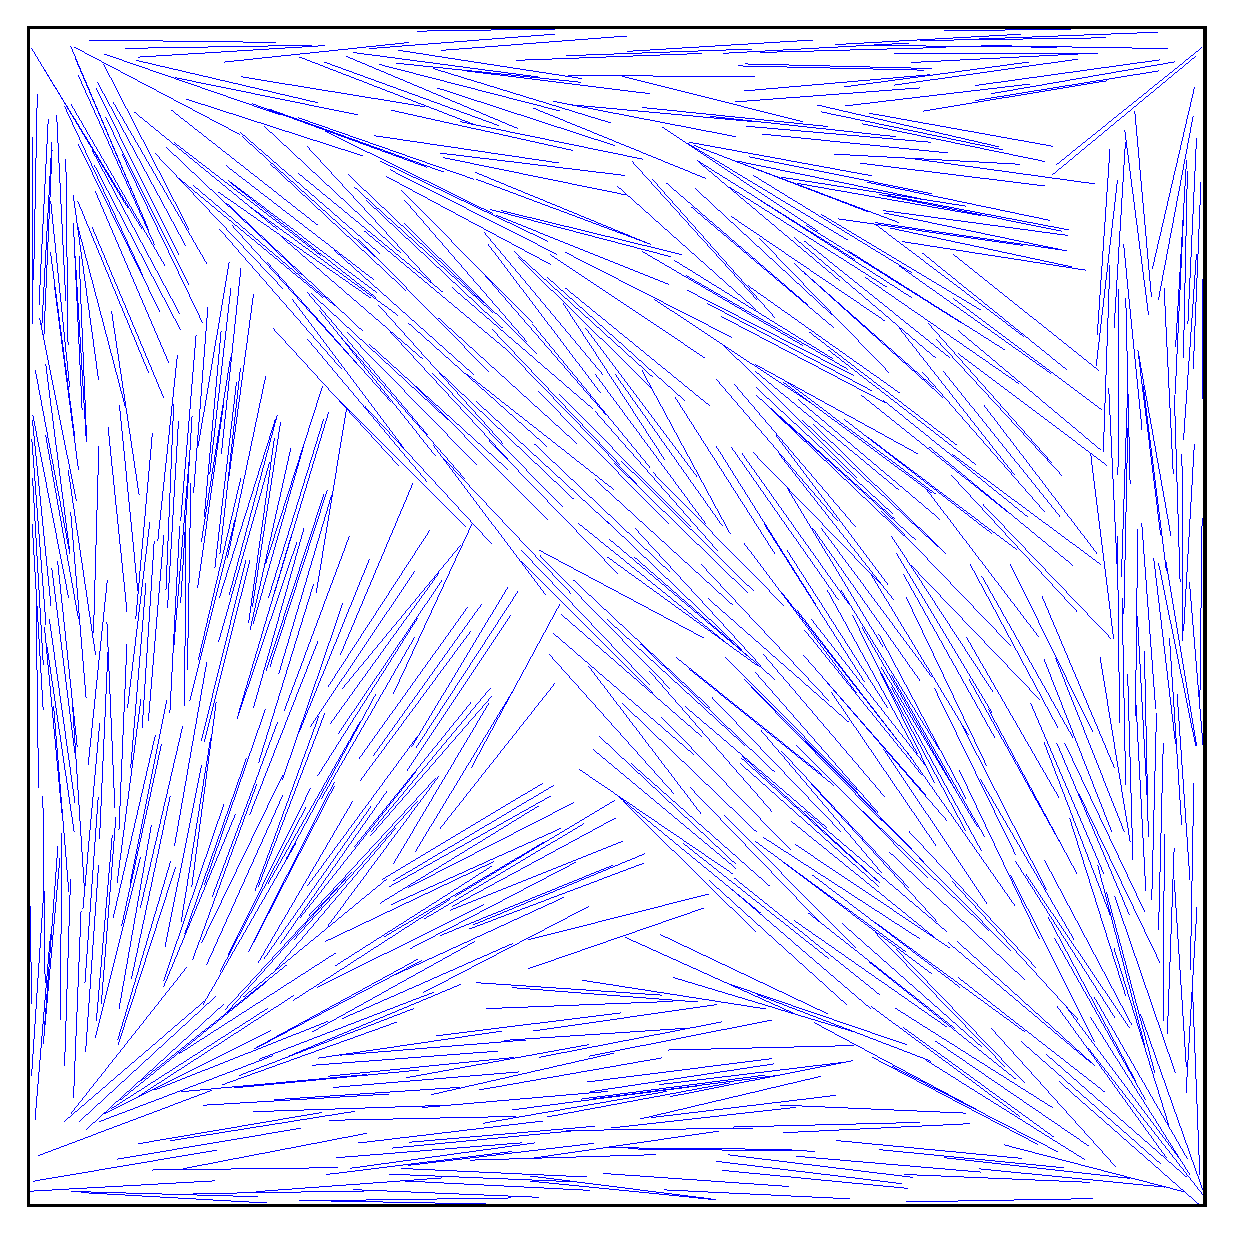
\includegraphics[width=0.9\columnwidth]{./figs/FIG1F.eps}\\
		(f)
	\end{minipage}%
	\begin{minipage}[t]{0.25\textwidth}
		\centering
		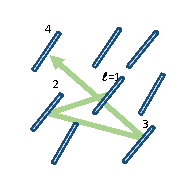
\includegraphics[width=0.9\columnwidth]{./figs/FIG1C.eps}\\
		(c)\\ \vspace{0.5cm}
		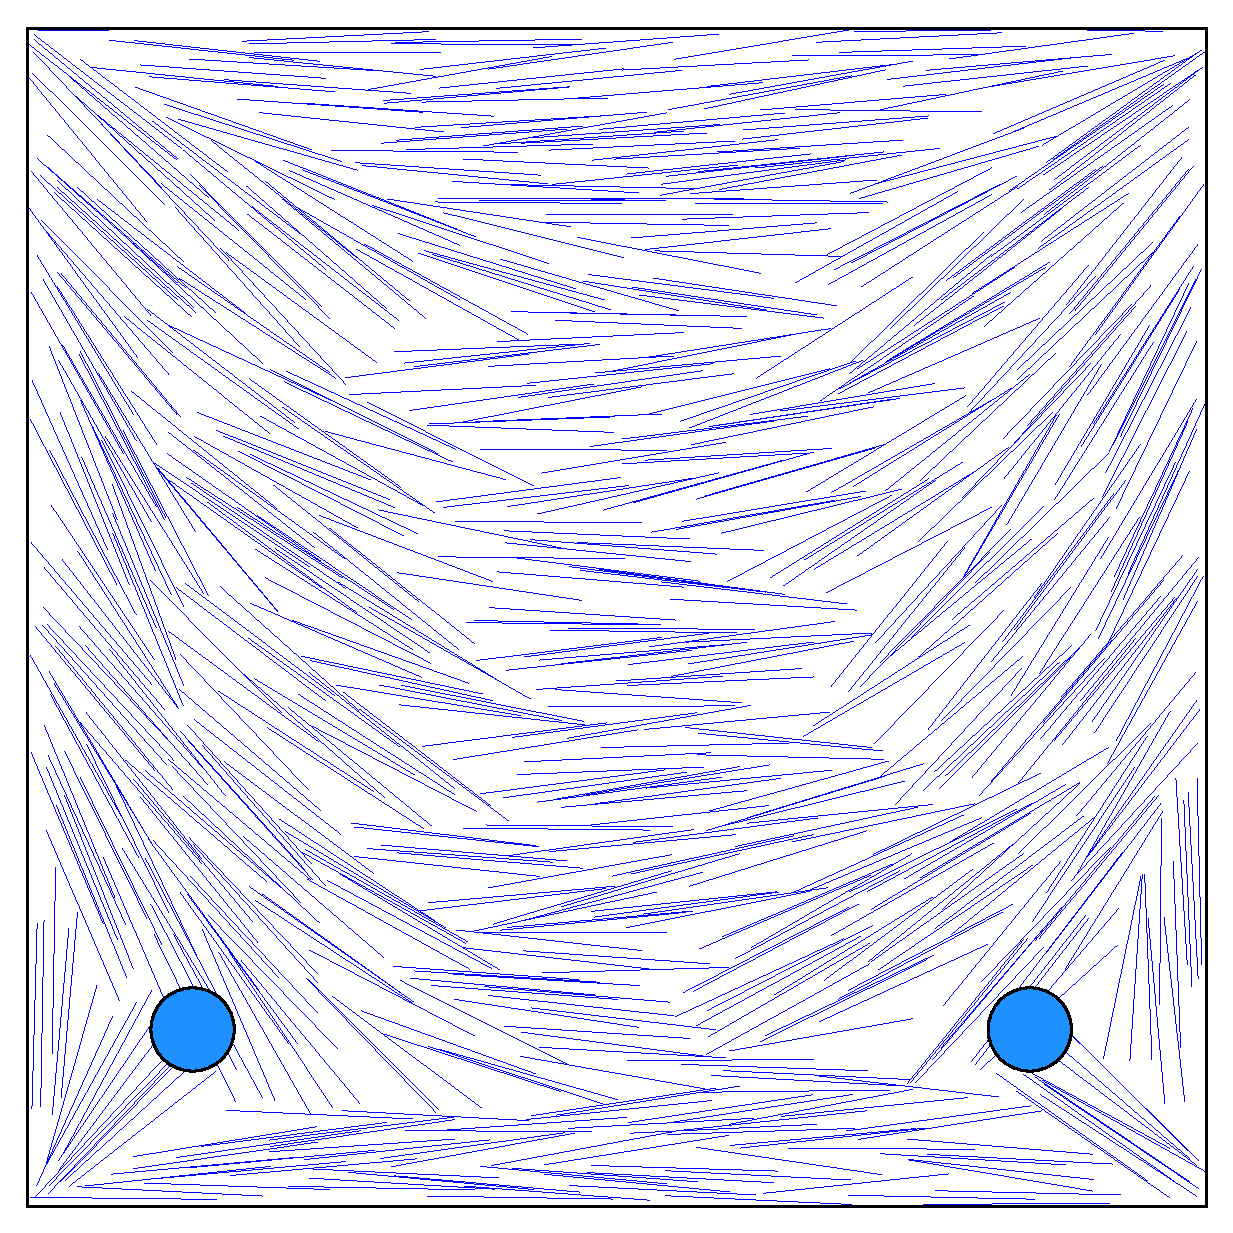
\includegraphics[width=0.9\columnwidth]{./figs/FIG1G.eps}\\
		(g)
	\end{minipage}%
	\begin{minipage}[t]{0.25\textwidth}
		\centering
		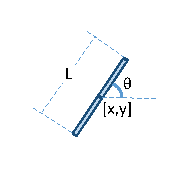
\includegraphics[width=0.9\columnwidth]{./figs/FIG1D.eps}\\
		(d)\\ \vspace{0.5cm}
		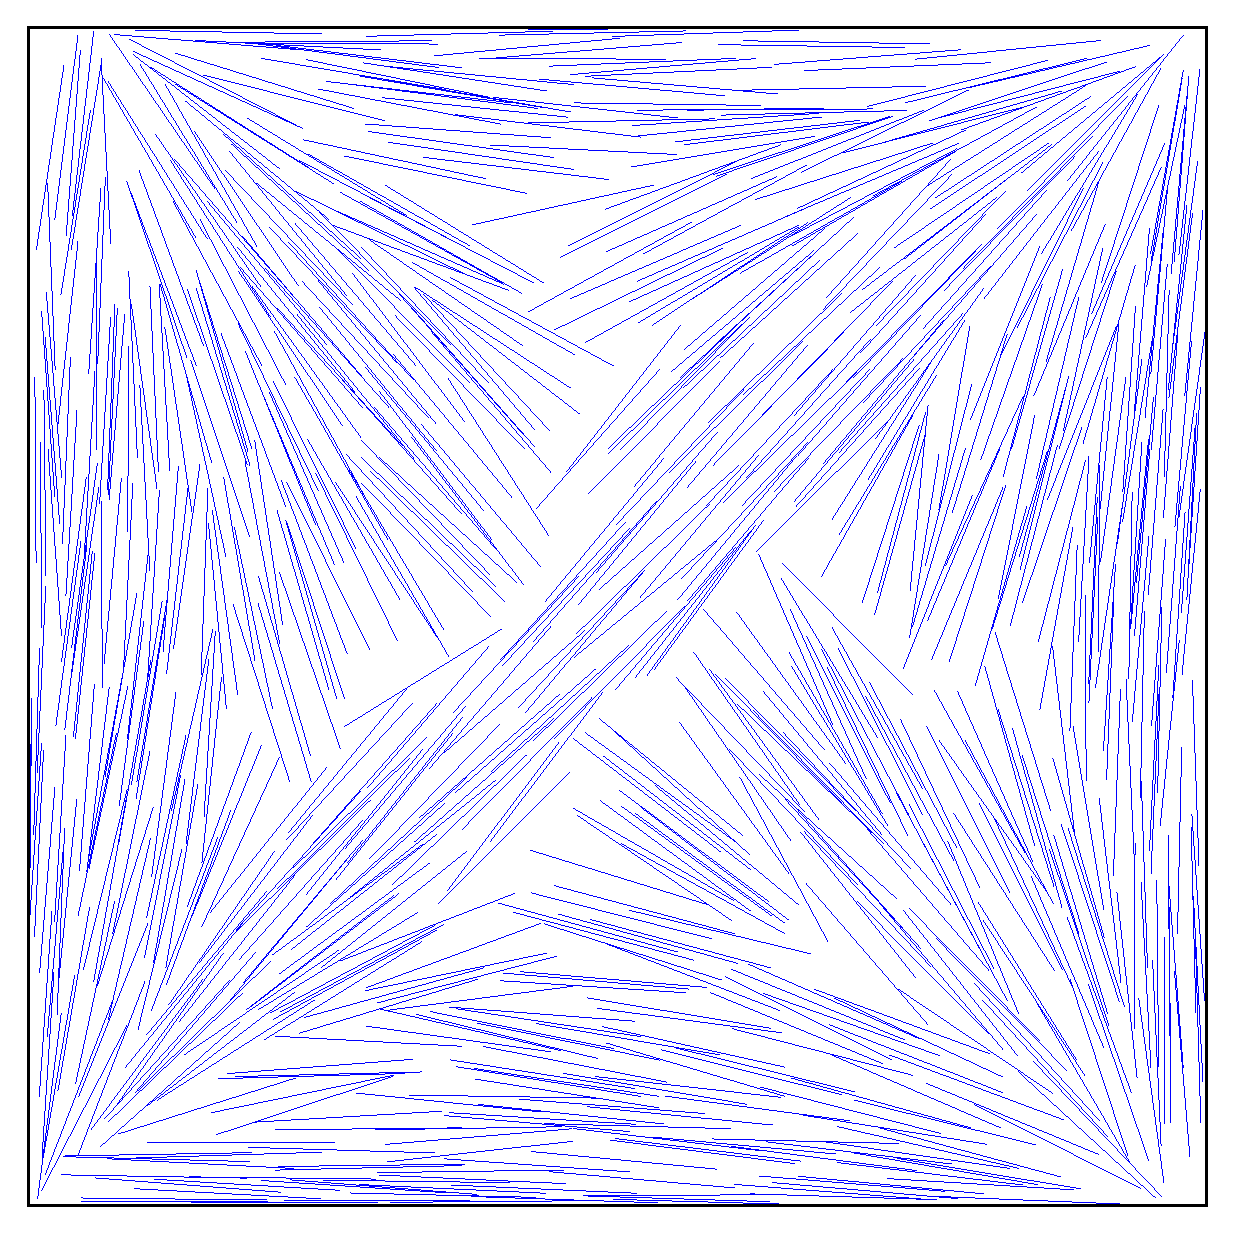
\includegraphics[width=0.9\columnwidth]{./figs/FIG1H.eps}\\
		(h)
	\end{minipage}%
	\caption{(a)-(d) Illustration of a two-dimensional hand-written image, Ising model, nematic state, and coordinates for a rod-like molecule,
		as well as (e)-(h) example configurations of different defect states generated from
		Monte Carlo simulations for a
		confined rod-like nematic fluid.
		The parameters used to generate these example configurations are $[N,a/L]=[784,6.32]$.
		The defect state in (e) has a diagonal (D) pattern, and
		the nematic textures in (f)-(h) resemble the tilted letter T, letter U, and letter X. The yellow and blue circles mark the defect locations of $-1$ and $-1/2$ winding numbers, respectively.
	}
	\label{FIG1}
\end{figure*}

One of the simplest neural networks is the feedforward neural network (FNN). A powerful tool, FNNs are able to accomplish a variety of image recognition tasks \cite{schmidhuber_deep}, a frequent benchmark test being the MNIST hand-written digit data set \cite{mnistset}. Figure \ref{FIG1}(a) shows one such digit from the MNIST set. Increasing the size and depth of a network boosts its ability to learn more complex patterns and features contained in images and then recognize these learned patterns in a new image.
An extension of the FNN, the convoluted neural network (CNN), has the network structure organized in such a way that local features of a pattern are dissected \cite{cnnmnist}.
CNNs have thus been a natural choice for condensed matter research, in particular problems on lattices such as the Ising model \cite{carras}, the XY model \cite{beach}, correlated fermions \cite{broecker,chng}, and other quantum systems.

In condensed matter physics we often deal with ordered states, where
certain physical features display spatial correlations in long range. Two typical examples are shown in Fig.\ \ref{FIG1}. In the ferromagnetic state, within an ordered domain spins align in one direction, as illustrated in Fig \ref{FIG1}(b). In the nematic liquid crystal state, within an ordered domain molecular directions are all aligned towards a common angle [Fig \ref{FIG1}(c)].
The images produced in these examples come from Monte Carlo simulations (see Appendix A for the current liquid-crystal system).
%%FNNs and CNNs are effective tools for identification of the disorder-to-ferromagnetic transition in the Ising model \cite{carras} and the isotropic-nemetic transition in the liquid crystal model [see Appendix B], when trained to recognize these different states.
Here, an ``image'' used for network learning is not a graphic image in the conventional sense. Rather, it is represented by the system configuration data containing physical features of each molecule (values of spins, angles specifying the orientations, etc).

These ordered states, on the other hand, sometimes have topological defects in their substantially ordered background. Different patterns can be characterized by different ways in which the local order parameters around the defects couple with the locations of the defects. Developing a characterization procedure to categorize these defects is a challenging task. A neural network (NN), then, becomes an ideal tool to identify these topological defects.
%
%In studying the Ising model with a neural network \hl{[IS THIS the paper for defect** We need to cite the defect paper here***]} \cite{carras}, an FNN was trained to recognize both high temperature (isotropic) states and low temperature (ferromagnetic) states. To read a given instance the neural net was given an ordered list of spins, from top-left to bottom-right. From this information alone the NN could learn the phase transition temperature, that is, it learned when contiguous regions were present or not.
%It would seem, then, the procedure is clear: a network with straightforward feeding of configurations through the input layer should enable the identification of defects in ordered states.
In studying the Kosterlitz-Thouless transition of the XY model \cite{beach}, a multilayered  network was trained on raw orientational configurations to learn the vortex unbinding that marks the transition. Accomplishing this requires the NN to understand topological features not too unlike the liquid crystal topologies in Fig.\ \ref{FIG1}(e)-(h). It would seem then that feeding the liquid crystal configurational data in a similar fashion should enable the identification of defects in ordered states.

However, we show here that such network structures are not readily appropriate for studying defect types of {\emph{off-lattice}} problems, such as the liquid-crystal defects shown in Fig.\ \ref{FIG1}((e)-(h)).
A typical configuration file generated from the computer simulations has a single-line data structure $[l,x_l,y_l,\theta_l]$ for a given molecule, where $l$ is the label of a molecule, and $[x_l,y_l, \theta_l]$ specify its $x$- and $y$- location coordinates and angular orientation [see Fig \ref{FIG1}(d)].
Because the molecules are allowed to randomly move in space, the label of a molecule, $l$, has no relationship at all with the spatial coordinates [see Fig \ref{FIG1}(c)].
This can be contrasted with a simulated data file produced by a lattice model. In such a case, positional information is already embedded in the order in which molecules are labeled (one naturally reads the data in the same order every time), as demonstrated by the arrow in Fig.\ \ref{FIG1}(b).
An NN that attempts to capture position-correlated patterns is thus implicitly aided from this direct mapping of physical position to the ordering of data in a lattice model.

Hence, we must solve how to capture the main features in a topological-defect state when the correlation between defect positions and the physical properties around them is the vital property. In this paper we discuss different ways of incorporating existing NNs for this purpose. As it turns out, an FNN (and conceivably a CNN) finds correlation between the order of appearance of data in the input and the physical features to be correlated. In an off-lattice model, index $l$ has no correlation with $[x_l,y_l, \theta_l]$. Even if we use $x_l, y_l$ as an input together with $\theta_l$, an FNN cannot find the correlation between $l$ and the input features $[x_l,y_l, \theta_l]$. This is discussed in Sect. \ref{FNN}.

Can we re-connect a relationship between $l$ and $x_l, y_l$ that can be easily used by an FNN for an off-lattice dataset? In Sect.
\ref{FNN} we develop and discuss a coarse-graining method which cuts the original simulation box into $m\times m$ equally sized cells where $m=1,2,4,8...$. The NN input is then ordered by cell index $M$, with the information inside each cell unordered. By such means, it is as though the system is approximated to a lattice form, with increasing accuracy as the cells become smaller and more numerous. An FNN can then begin to correlate physical features with position and identify topological defects with appropriate cell size.

However, we present another more general method, using a recurrent neural network (RNN), that avoids the need for any presorting.
The RNN is a neural network specialized in correlating sequential information (e.g.\ analyzing a time series of images \cite{rnnvideo}, or predicting upcoming words in a sentence based on previous words \cite{rnnwords1,rnnwords2}). In Sect. \ref{RNN}, we propose a scheme to feed
$x$, $y$, and $\theta$ data sequentially, akin to three time sequenced images, which enables the RNN to correlate these three features. Turning temporal correlation to spatial correlation, an RNN can efficiently identify different states in the original raw data, without any of the coarse-graining or presorting needed for the FNN.

We selected the topological defects appearing in the system of $N$ rod-like molecules confined by a square boundary in two dimensions (2D) as a
vehicle to deliver the concepts in this paper. This system has been the focus of recent theoretical and experimental studies due to its practical relevance \cite{Galanis2006,Mulder2011,Lewis2014,Cortes2017} and interesting theoretical aspects \cite{Tsakonas2007,Luo2012,Chen2013,Mulder2015,Lewis2014,robinson2017,yao}.
For example, %in Refs. \citen{yao,robinson2017}
the possible defect states were recently studied in-depth in terms of
the continuum Landau-de~Gennes model \cite{robinson2017} and
the Onsager model \cite{yao},
producing a comparable ensemble of stable and metastable states as
the result of minimizing the free energies in
these different models.
Our aim here is not a detailed study of this particular liquid crystal system, to which we direct the readers to the above references for more details on their significance and origin.
Rather, we selected four major defect states, D, T, U, and X, shown in Fig.\ \ref{FIG1}(e)-(h), for use in our machine learning study on the molecular data files. For this purpose,
we developed a Monte Carlo algorithm to produce the necessary data.
The computer simulation procedure, as well as the system's isotropic-nematic transition properties, are explained in Appendices \ref{MC} and \ref{IN}.

The location of the nematic defect points are indicated in Fig. \ref{FIG1}(e)-(h) by colored circles. Here we see only two types of defects: those with winding number $-1/2$ (blue) and $-1$ (yellow). Although one could argue that the defects are point-like local objects, in a finite system, the overall nematic ordering in separate bulk areas are strongly connected with these local features. Each topology has a unique arrangement of the defect locations and overall nematic texture.


%Robinson \etal \cite{robinson2017} also provide an in-depth look and comparison using several numerical methods (off-lattice, on-lattice, continuum) of our same 2D square-confined LC system. Their alternative Landau-deGennes continuum model also found many of the same states the Onsager model produced in \cite{yao}.\\

Returning to the classic example of identifying hand-written numerical digits from 0 to 9, we make a comparison between the darkened pixels in this case with the topological defects in our confined liquid crystal system. In a sense, what a neural network looks for is the feature correlation of the spatial position of the darkened pixels in these images. In Appendix \ref{AppMNIST}, we re-enforce some of our concepts mentioned above, by treating the digit recognition problem as a defect state identification problem.
%When it comes this classical application the question must be asked: To order or not to order?

This work is motivated by the question of whether machine learning can be used to identify topological defects, which in this case are those of confined two-dimensional liquid crystals. We clearly make recommendations on data handling and
the choice of neural network, suitable for defect identification; these can form useful steps for  more general problems in studying other condensed matter systems, in particular, data generated from off-lattice models.

\begin{figure}
	%\centering
	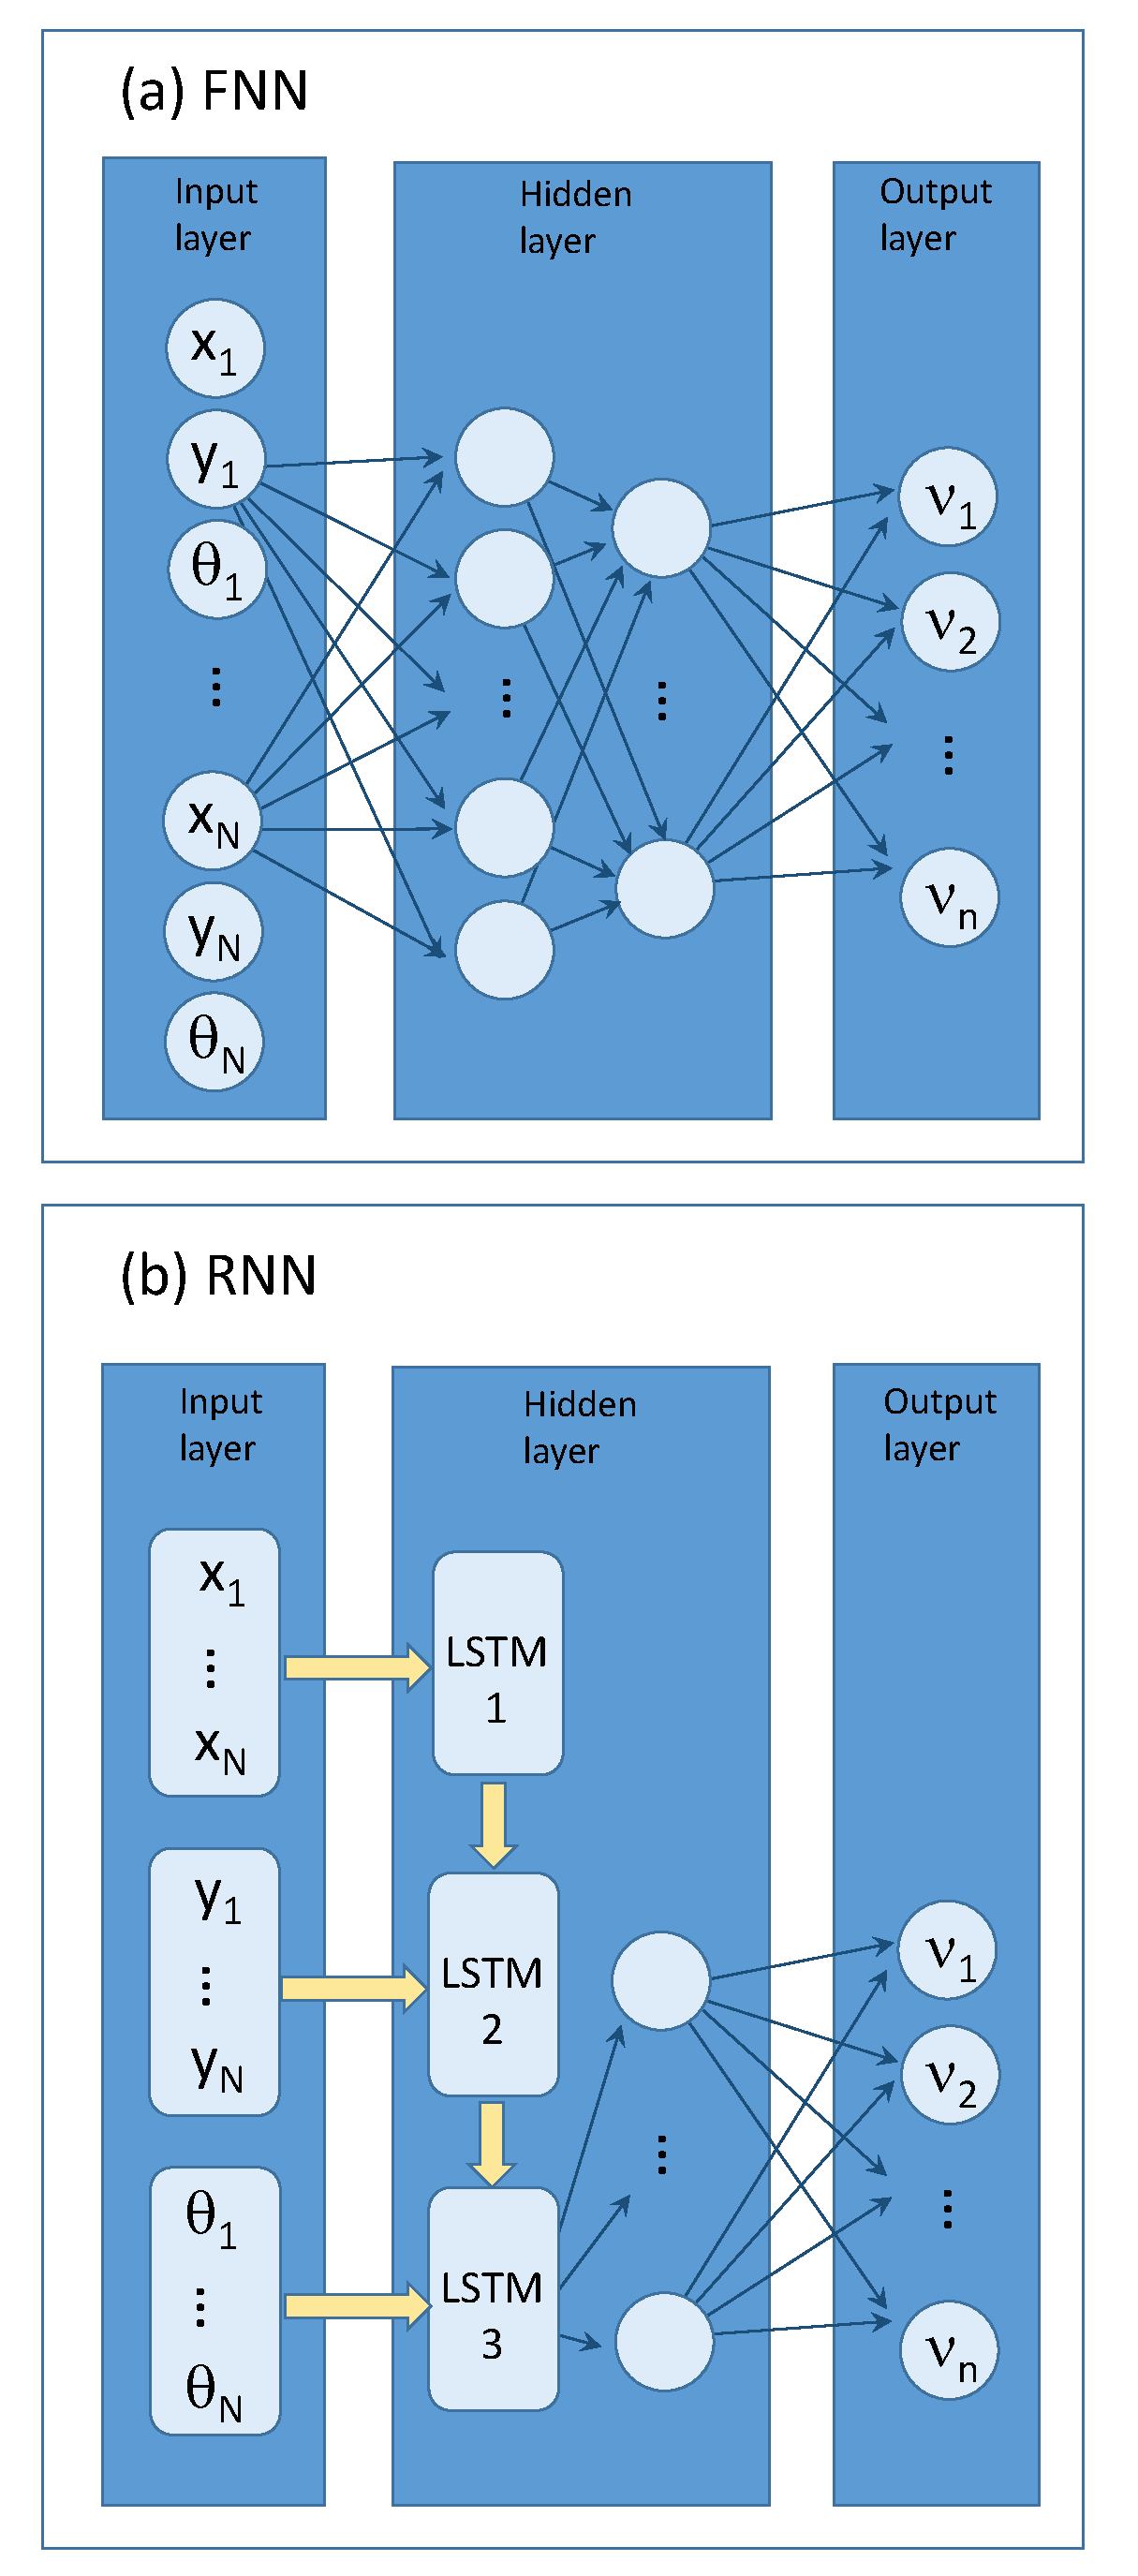
\includegraphics[width=0.8\columnwidth]{./figs/FIG2.eps}
	\caption{Schematics of (a) an FNN with two hidden layers and the sequence $(x_l, y_l, \theta_l)$ as input, where $l=1,2,...N$, and (b)
		an RNN (unrolled) with the sequence $x_l$ ($l=1,2,...N$) as the input to the first LSTM block,
		$y_l$ ($l=1,2,...N$) to the second LSTM block, and $\theta_l$ ($l=1,2,...N$) to the third LSTM block.
		LSTM blocks also have LSTM-LSTM connections.
		The final output of the two networks are $\nu_1, \nu_2, ..., \nu_n$, where $n$ is adjusted according to the type of features to be identified.
	}
	\label{FIG2}
\end{figure}


\section{Preparation of the training and testing data}\label{TrainingData}

The physical system studied here is the defect states generated from the MC simulation of a two-dimensional off-lattice liquid-crystal model.
In total, $N=784$ rod-like molecules of length $L$ are confined to a square box of dimensions $a\times a$.
Mutual crossing of rods and crossing of box boundaries by rods are forbidden to simulate the excluded-volume interactions. Monte Carlo details can be found in Appendix \ref{MC}.

One can show that the parameter that drives the phase transition is the reduced density,
\begin{equation}\label{rho}
\rho \equiv \frac{NL^2}{a^2}.
\end{equation}
Above the critical value $\rho^*$ the system is in a nematic state with directional ordering and below the critical value the system is in an isotropic state with random orientations (except those near the walls). The critical density $\rho^*\simeq 6.71$ can be estimated from a typical machine learning application, described in Appendix \ref{IN}.

Our main concern here is identifying the defect states, not the isotropic-to-nematic phase transition itself.
Within the nematic state, the system can display a stable D-defect pattern, or can be trapped in the free energy minima corresponding to one of the X-, T-, or U-defect patterns, due to the finite confinement effects. The nature of the metastability has been recently addressed extensively in Refs.\ \cite{Galanis2006,Mulder2011,Lewis2014,Cortes2017,Tsakonas2007,Luo2012,Chen2013,Mulder2015}.
In order to explore the best machine learning techniques in identifying the defect states, we established a database from the MC simulations at a fixed  $\rho=19.63$ (produced by setting $a=6.32L$). The relatively high $\rho$  enables the trapping of the metastable defect patterns during simulation runs.
In total, $4400$ independent configurational snapshots were collected for each of the defect states [see Appendix \ref{MC}].
Of these, $400$ snapshots were reserved for the testing dataset.

%
%To build up datasets a relatively high density of $\rho=19.63$ was used so the different defect patterns could maintain their form as they are metastable at lower densities. For each pattern $4400$ independent snapshots were collected [see Appendix \ref{MC}].

For each defect type in Figs. \ref{FIG1}(e)-(h), $4000$ snapshots were used for training. A typical defect pattern can be rotated by a $\pi/2$-, $\pi$-, or $3\pi/2$-angle and maintains its topological structure, because of the square boundary geometry. Since these $4000$ snapshots were taken from MC simulations, they already contain all different orientations of the defect pattern naturally. To ensure that all four orientations of the square boundary are indeed equally treated, we further rotate these $4000$ snapshots by these angles.

The raw dataset of each snapshot contained coordinate data ordered by the label of molecules, $l$, and followed by $[x_l,y_l,\theta_l]$ [see Fig. \ref{FIG1}(d)], where $l=1,2,...,N$. The treatment differs from the pixel approach of a digital image, for which a pixel grid system would be established.



\section{Application of FNN}\label{FNN}


First we review a few basic neural network concepts.
The main function of an NN is to read the system configuration through an input layer (e.g.\ an image, text, or sound bite), process the information in  hidden layers, and then generate an output. The output is often a classification estimation of the input, but may be another data structure (another image or sound bite for instance). In our case we look to classify system states through an FNN, sketched in Fig. \ref{FIG2}(a).
Each arrow (an ``edge'') represents a function call that connects nodes in different layers. These nodes, or ``perceptrons'', are inspired by the neuron model of the brain and are the building blocks of many neural networks, including the FNN, and though individually quite simple, complex functions can be represented by networking many perceptrons together \cite{rosenblatt}.
Going from input to output, data is repeatedly manipulated through function calls at each layer, with each containing their own network parameters --- usually referred to as weights and biases.
By varying network parameters the final output is consequently affected.
Training a network then involves optimizing the network's performance in producing the desirable output with respect to these network parameters.
%Multiple ``epochs'' are needed during the training, where w
Within one ``epoch'' the network is trained once on the selected dataset, and in general multiple epochs are needed for a network to converge to an acceptable performance.

A few technical details are provided.
We used a multilayer perceptron FNN of modest size, having two hidden layers: the first of size 128, and the second of size 32.
With the implementation of Tensorflow, exponential linear units were the chosen neurons for their proven effectiveness and quick learning \cite{elu,tensorflow}, and an early stopping technique determined sufficient training time \cite{nntricks}. Dropout was used at a 50\% drop rate to reduce overfitting the training \cite{dropout}.
The Adam algorithm was used for optimization \cite{adam}, and Softmax was applied to the output neurons to normalize the output set [see Appendix \ref{Supervise}].
For evaluating NN performance, a separate test dataset of images not seen during training is needed. A useful NN model needs to be able to correctly classify images it has not been trained on, otherwise it may merely have found a set of parameters that only work for the training set.

We used cross entropy $S$ as the cost function to measure the training quality on the training data set;
plotted as a function of epoch, we can see how the model learns over time and estimate its learning trajectory.
When the network is adequately trained, $S$ approaches 0. Another unique insight into the network's performance is the accuracy $A$, defined to measure the network performance on the unseen test set. An accuracy of 1 is scored for correct classification on the entire test set. Both $S$ and $A$ are quantitatively defined in Appendix \ref{Supervise}.

%The MC parameters for the DTUX sets were chosen so as to be in a favorable region for both $U$ and $T$ states, as predicted by Yao \cite{yao}. We chose a box size of edge length $a=6.32$, rod length of unity, and number of rods $N=28^2$, yielding a reduced density $\rho^*=19.63$. This region, though favorable, was still only metastable and relaxing for much longer than $10^5$ Monte Carlo sweeps (where one sweep attempts to move each rod) would inevitably tend towards the more preferred D state. In accounting for this, after $10^5$ sweeps, the state snapshot would be recorded, the system would be reinitialized, and the process would repeat. This additionally ensured no temporal correlation among snapshots.

A naive approach would be directly taking an FNN for identifying these defect states, sequentially feeding the raw $[x_l,y_l,\theta_l]$ data into the $3N$ input nodes, and training the network to recognize the four different topologies by supervised learning [see Appendix \ref{Supervise}].
This approach has seen success in learning phase transitions of Ising systems \cite{carras}, polymer systems \cite{wei}, and the XY model to a degree \cite{beach}. However, this method showed a pronounced failure in the current application.
As we show in Fig.~\ref{xtud-all}(a), indicated as $m=1$, this approach does not come close to an acceptable performance, producing a plateau in an undiminishing cost. In addition, $A$ reaches a plateau at an unsatisfactory level of approximately $60\%$.

Why is this so?
One of the essential features the network needs to learn for these defect configurations is the correlation between the position of a topological defect and the molecular orientation in the vicinity of the defect. A typical raw snapshot datafile records the $[x,y,\theta]$ data sequentially according to the order of the label of the rod-like molecules $l$. Because there is no a priori knowledge of which molecules show up in the defect regions, the labels of the defect-region molecules differ from file to file. Indeed, in a statistically independent set of files, such as the ones produced here from different initial conditions [see Appendix \ref{MC}], there are no label-position correlations of the defect-region molecules among the learning data files.
This all addresses a crucial, but often unappreciated, aspect of image classification: by filling input vectors in a positionally sorted fashion [Fig.~ \ref{FIG1}(a),(b)], positional information, and indeed its correlation to whichever feature is being written to the input vector, is consequently encoded. If this sorting is destroyed, even if we give the positions (such as $[x,y]$
) as part of the input data, the position-feature (e.g.\ $\theta$) correlation is destroyed. This unseen property, and its essential importance can also be demonstrated via the digit recognition problem in Appendix \ref{AppMNIST}.

Hence, the key information is the position sorting in the initial data input, as the FNN relates features with the ordering of the input data. We develop the following coarse-graining procedure to train an FNN in identifying liquid crystal defects shown in Fig.~\ref{FIG1}.

The confinement box (Fig.~\ref{FIG1}) is divided into $m\times m$ cells, where $m$ is an integer. The cells are labeled $M=1,2,...m\times m$ horizontally, row by row.
The raw data in every snapshot is consequently presorted according to
the center-of-mass coordinates of the molecules, $[x,y]$, so that molecules belonging to the $M=1$ cell show up first, $M=2$ cell show up second, etc. Within a cell, the order of data is still random and no further presorting is made.
Even if a rod extends into multiple cells, the fixed input vector allows it only to appear once. The center of mass of the rod makes a natural choice.
The $m=1$ case returns to the raw data format. By the end, the order of appearance of molecular information is no longer according to $l$, but, according to $M$ for all coarse-graining degree $m\ge 2$. The presorted data is then used in supervised training.

The presorting procedure works well with an FNN. Figures \ref{xtud-all}(a) and (b) show how the cost function and accuracy quickly approach the ideal value of $0$ and $1$ respectively, as we presort the data beyond $m=2$.
In the case of $m=4, 8$, less than 20 epochs (surprisingly short) are needed to adequately train the FNN. This can be attributed to the defect patterns in Fig.\ \ref{FIG1} themselves. By dividing the square box in $m=4$ cells, for example, one can already distinguish the defect structures, by ignoring fine details inside a single cell.
Of course,  in general we expect that the degree of coarse-graining, $m$, needs to increase for a more complicated defect pattern with more defect features.

In summary, to effectively train an FNN to identify features in an image or simulation data file, the ordering of data points (pixels in image, spins in the Ising model, and rod-like molecules in the current study) contains vital information of the data. An off-lattice model usually produces data with a random order and it must be presorted according their approximate $[x,y]$ coordinates, if we are looking for the correlation between coordinates and the physical features.



\begin{figure*}[]
	\centering
	\begin{minipage}[t]{\columnwidth}
		\centering
		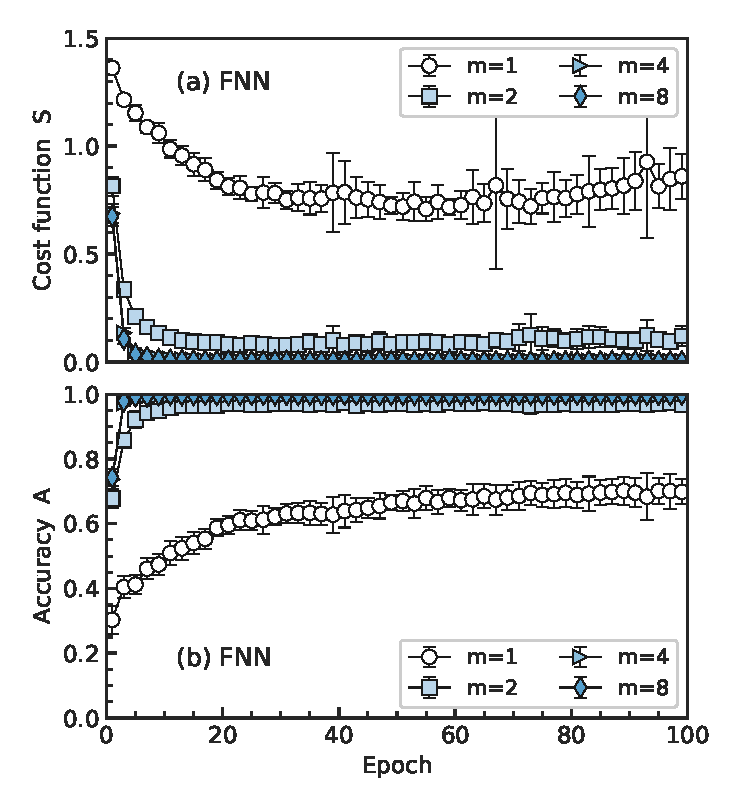
\includegraphics[width=\textwidth]{./figs/FIG3AB.eps}
	\end{minipage}%
	\begin{minipage}[t]{\columnwidth}
		\centering
		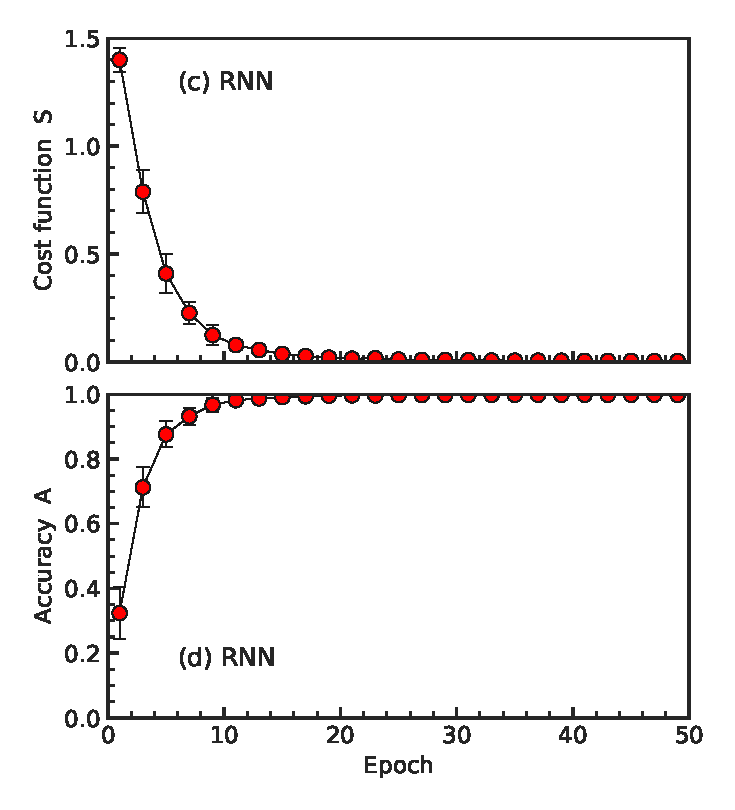
\includegraphics[width=\textwidth]{./figs/FIG3CD.eps}
	\end{minipage}
	\caption{Cost function $S$ and accuracy $A$, defined on the training and test datasets respectively, monitored on an FNN [(a) and (b)] and RNN [(c) and (d)] as functions of epoch step. Symbols in the plots represent the averaged $S$ and $A$ produced from 20 repeated training runs, from which errorbars are also estimated. Circles, squares, triangles, and diamonds in (a) and (b) correspond to the degrees of coarse-graining in the presorting procedure used: $m=1$ (unsorted raw data), $2$, 4, and 8, respectively. For coarse-graining, the original simulation box in Fig.\ \ref{FIG1}(e)-(h) is divided into $m\times m$ cells [see Section \ref{FNN}]. The circles in (c) and (d) also represent the same averaged $S$ and $A$, where an RNN was used with raw, unsorted data as the input (i.e., $m=1$).
	}
	\label{xtud-all}
\end{figure*}


\section{Application of RNN}\label{RNN}

A typical structure of the recurrent neutral network (RNN) is represented in Fig.~\ref{FIG2}(b). The crux of this RNN is the long short-term memory (LSTM) cell module \cite{lstm}. An RNN can be made with different types of modules, but the LSTM is a popular choice and is well-sufficient for this work. Except for the first block, an LSTM cell has two input channels: an LSTM-external connection
to new raw data from the system to be studied,
and an LSTM-LSTM connection, taking its own output and internal weights from the previous step as input, hence the recurrent aspect. Schematically, it helps to represent this as a series of LSTM cells for each raw data input.
To complete the RNN, a single layer of perceptrons is appended to act as
a final interpretive layer of the LSTM output, compressing the large LSTM output to the smaller prediction output $(\nu_1, \nu_2, ..., \nu_n)$.

RNNs initially gained popularity for time series applications. An LSTM cell can take a complete data file and at each iteration of input, consider the new raw data together with its own previous state simultaneously. That is, an LSTM establishes data correlations with those fed into earlier cell states through LSTM-LSTM connections.
%A popular application of RNNs is speech recognition, where a long series of connected LSTM blocks are used; if one uses $i$ to denote LSTM blocks sequentially, then the input to the $i$th LSTM block is a complete dataset occurred at time frame $t_i$; the time series $...t_{i-2}, t_{i-1}, t_i$ of a speech record can then be processed with time-correlation.
In its composition, like an FNN, an RNN (including the LSTM) is still merely an ensemble of floating-point network parameters.
The logic of supervised training is the same here as with an FNN: determination of the network parameters through optimization of a cost function. The RNN can be coded in terms of Tensorflow libraries efficiently.


Here we demonstrate a novel usage of an RNN in condensed matter systems. Exploiting its ability to correlate physical features through LSTM blocks, we adopt a triple iterative structure shown in Fig.\ \ref{FIG2}(b) to find the correlation between the spatial coordinates $x$, $y$ and the orientational coordinate $\theta$. The raw Monte Carlo data has a line-by-line format $[l, x_l, y_l, \theta_l]$, where $l=1,..., N$. The three main features, $x_l, y_l$ and $\theta_l$ are input into the network model iteratively through the LSTM-external layer, one after another. As a technical note, we used a rather small RNN having only a single layer LSTM of 64 hidden neurons, and a single perceptron layer of 128 neurons. Dropout, Adam optimization, and early stopping were again used throughout the supervised training \cite{dropout,nntricks,adam}.

The performance of this RNN is exceptionally good in identifying the defect states. Figures \ref{xtud-all}(c) and (d) demonstrate that within an initial 20 epochs, our RNN efficiently captures the main features of the four defect states, evaluated on an unseen test dataset. We stress here that unlike the procedure used to produce Figs. \ref{xtud-all}(a) and (b), we used the raw, unsorted data as the input on our RNN experiment. 

Another use of keen interest would be detecting which types of nematic defects (usually represented by a winding number) are present and their locations in a larger nematic image.
The current approach of using the entire configuration data in RNN is not ready for this task but we could certainly extend our method for this purpose. We can divide the large nematic image into appropriately small cells, and use the data in each cell as the input for RNN.  Using supervised learning in much the same way as this study, the RNN could be trained to recognize a defect cell versus a normal cell; then, in an application stage, 
the trained RNN can be used to sweep through the entire image and identify the type and location of a defect cell. Future study in this direction is needed.


Without other analysis tools it is difficult to say which \textit{exact} topological features the RNN is learning to distinguish the XTUD image set.
One could argue that the
location of a defect in a larger system is a point-like object, but the XTUD topologies here, complete in their square confinement, are compositions of bulky nematic patterns interrupted at defect points [Fig.~\ref{FIG1}(e)-(h)]. In a finite system such as the one we take here, the exact division between defect points and the overall nematic pattern becomes artificial.
We intend to believe that the RNN examines their entire topologies
by correlating the spatial-angular information.

Beyond liquid crystals, many other classes of materials contain topological defects that are of practical or fundamental interest; some are detectable by the naked eye and some are subtle to visualize. Especially when a molecular configuration file is given, either produced directly from computer simulations or indirectly reproduced from real experiments, the fluctuating microscopic configurations of all molecules could obscure the existence of a certain topological feature. Hence it would be desirable to have a computer algorithm to deal with the nontrivial task of identifying these states.

In order to design a classical algorithm to identify the topological states, understanding the main features (spatial dimensionality, line defect versus point defect, definition of winding number, etc.) is required to describe a specific nature of the state. Well-thought mathematical procedures would be needed to capture the correlation (or discorrelation) between defect regions for different states.
Classification would then require tools that identify defects, locate them reliably, and finally try to correctly classify this to their human-defined templates.
The NN model here presents a universal and simple method that sidesteps this non-trivial process by requiring only the raw data as input. 
The RNN can masterfully learn these defect topologies by using its ability of making correlations between data features, without asking the question of the specific mathematical and physical properties such as where to look for the defects and what kind of defects a system may contain.

The neural network approach we suggest here is simple, automated, and universal.
%While these are advantages, they could be disadvantage as well.
%It is well known that often machine learning gives us excellent characterization accuracy but a very poor understanding of how such characterizations are made. In a scenario where we do not need to understand which distinguishing features end up being important, our current approach works well. In a different scenario where a single few features stand out, further studies are needed for capturing these, especially for an off-lattice system.
Additionally, neural nets can provide a near instantaneous computing time for classification, of course minus the time required for training. In our case though, this was agreeable, requiring only tens of minutes.


\section{Summary}

In this paper, we examined the ability of an FNN and RNN in learning and identifying the topological-defect configurations produced from Monte Carlo simulations of a liquid-crystal model. The predominating physical characteristics of the defect pattern is the positioning of defects and its coupling with the nematic pattern around the defects. Our main conclusions include: for effective learning with an FNN the simulation data must be presorted to restore the data ordering of spatial information, and with an RNN no such presorting is needed.

Exploiting the RNN capability to correlate spatial features (such as the topological defects) in their sequential inputs is a novel use here.
Our study opens up opportunities for many other off-lattice applications of neural networks. By iteratively feeding an RNN with features to be correlated, it is able to correlate arbitrary numbers of interested features of an off-lattice problem. This is particularly important as off-lattice simulations usually produce datasets with no embedded spatial ordering, whereas lattice simulations automatically have spin labels implicitly representing spatial locations.



\section{Acknowledgement}
We thank the Natural Sciences and Engineering Research Council of Canada for financial support and Compute Canada for providing computational resources.



\section{Monte Carlo Simulation}\label{MC}
%[A list of several papers using ml and MC: \cite{huang,portman,liu,torlai}\\

In order to generate the data pool to train our neural networks, we adopt the Monte Carlo simulation method that generates configurations of our molecular-level model. The simulated system contains $N$ rigid rods, each having length $L$, confined to a 2D square area of side-length $a$. In 2D, a single rod can be represented by a straight line, described by the center-of-mass coordinates, $[x, y]$, and the direction that the rod  makes with respect to the $x$-axis, $\theta$ [see Fig.\ \ref{FIG1}(d)]. No rod thickness is considered here, as in a 2D space, two infinitesimally thin rods already interact with each other by an excluded ``volume'', namely, an excluded area. A successfully generated configuration contains the $[l, x_l,y_l,\theta_l]$ coordinates of all $N$ rod-like molecules, line by line for $l=1,2,3...N$. The wall-confinement effect is enforced by disallowing the intersection of a rod-like molecule with the wall boundaries. Although the macrostate of a system is specified by three parameters $N$, $L$, and $a$, only two are relevant, $N$, and $L/a$.

A typical MC attempt of a randomly selected molecule consists of a translational move by changing $[x, y]$ and a rotational move by changing $\theta$ about the rod center of mass. These moves are
realized by adding a coordinate shift within the range $[-\Delta, \Delta]$ (for the former) or an angular shift $[-\delta, \delta]$ (for the latter). Any moves that violate the excluded-area constraint and the boundary conditions are rejected. The magnitudes of $\Delta$ and $\delta$ are determined by trial and error to maintain acceptance rates close to $50\%$ \cite{Landau}, independently for the translational and rotational moves, to allow sufficient system evolution. An MC step (MCS) pertains to making $N$ MC attempts (one for each rod on average) described here. To speed up the simulation, the cell-index technique \cite{allen} was incorporated in the algorithm.

%For a specified set of parameters, $N$ and $L/a$, an initial configuration was generated by placing the rod-like molecules inside the box as a lattice with equal spacing, without concerns of the excluded-area interaction and the boundary conditions. The orientations of the rods would be purposely distributed according to the desired defect configurations. Since we used supervised learning with labeled images, the system had to be in a known configuration. After this, each rod was given small random positional and orientational nudges to add some randomization. A rod-uncrossing period of the MC simulation would follow; typically for density $\rho \sim 16$, this period was approximately $5\times 10^4$ MCS.

%The configuration data for the X, T, and U states were collected by using a modified method. Because the these are ``thermodynamically'' metastable configurations, a simulation run of a denser system has the tendency to trap these states for a longer time.
All the DTUX data sets had $N=784$ rods and a box-edge to rod length ratio $a/L=6.32$, amounting to a density $\rho=19.63$. The relatively high density ensures the lifetime of metastable XTU states.
%These defect patterns, in their own rights, could be stable and metastable. Going from a metastable state to a stable state could take forever in a Monte Carlo simulation.
Trapping of a particular type of defect state depends on the initial condition. We take the approach of randomly placing rods in the box to start with and then align the directions of the rods according to a particular defect pattern. After this, each rod was given a small random positional and orientational nudge to add some randomization. Generally, there would still be substantial crossing between the rods and between rods and walls.
An uncrossing MC period was then conducted; typically for density $\rho \sim 19$, this period was approximately $5\times 10^4$ MCS.
After that, the systems were run for $10^4$ MCS to further equilibrate the system. This was followed by taking a ``snapshot'' (i.e. writing the rod coordinates and angles to a file). For each topology, $4400$ snapshots were taken from independent runs, each having a different initial condition from the random nudging. Among these, $4000$ snapshots were used for training and $400$ set aside for testing. To cover rotational degeneracy of the topologies, an equal number of images were rotated $\pi/2$, $\pi$, and $3\pi/2$.
\\



\begin{figure*}[!t]
	\centering
	\begin{minipage}[t]{0.9\textwidth}
		%		\centering
		{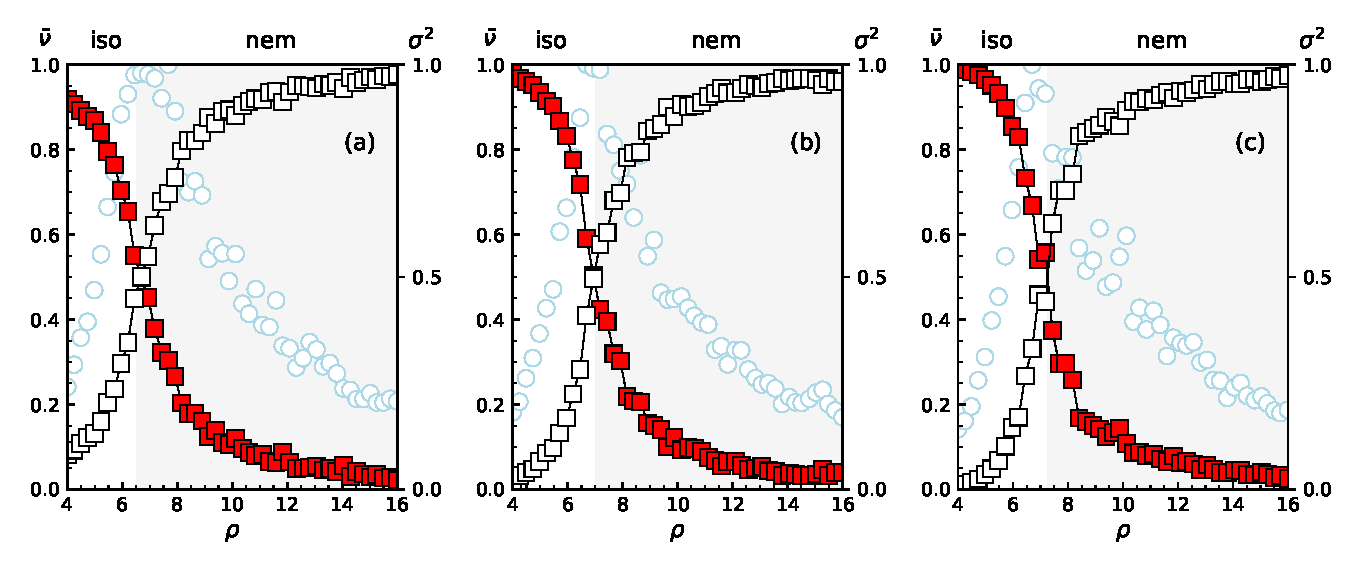
\includegraphics[width=\columnwidth]{./figs/FIG4.eps}}\\
		%		\vspace{-0.5cm}
		%		\begin{flushleft}
		%			\hspace{0.18\textwidth} (a)
		%			\hspace{0.29\textwidth} (b)
		%			\hspace{0.285\textwidth} (c)
		%		\end{flushleft}
	\end{minipage}%
	\caption{Identification of the I-N transition point. An FNN is trained by using training files at low and high densities ($\rho=4$ and 16 for the I and N states, respectively).
		Then, the trained FNN is used to calculate the average outputs $\bar{\nu_1}$ and $\bar{\nu_2}$ at each given $\rho$. These characteristic measures are to indicate if the system is in an I or N state, plotted by red and white squares, respectively.
		Error bars of these data points are smaller than the symbols sizes. The crossing point is defined as the I-N transition point. In the background, represented by circles (to the right scale), an independent estimate of the variance of the orientational order parameter $\sigma^2$ (normalized), shows a peak at the transition point. Blue and white circles represent the statistics from rods in the entire box and half-sized center region, respectively.
		The three plots, (a), (b), and (c), are produced with system sizes
		$N=20^2$, $24^2$, and $28^2$, respectively.
	}
	\label{fnn}
\end{figure*}

\section{The isotropic-nematic phase transition and FNN}\label{IN}

%The molecular configurations of the current system is typically represented by the coordinates and orientations of the $N$ rod-like molecules of length $L$, within a confining square box of dimensions $a\times a$. Two control parameters then emerge in the current system. One is the reduced molecular density,
%\begin{equation}\label{rho}
%    \rho = NL^2/a^2,
%\end{equation}
%which controls the system to stay in an isotropic or nematic states. The ratio $L/a$ is another parameter, particularly relevant in the $L/a  \lesssim 1$ regime. Together with $\rho$, it also controls which type of defect patterns that can be stabilized.

In this work, we used the off-lattice model of rod-like molecules confined in a square box as an example of a system containing topological defects in its nematic state. The dominating physical parameter is $\rho$. Above a critical value $\rho^*$, the system is in the nematic (N) state showing a defect pattern such as those in Fig.\ \ref{FIG1}, and
below $\rho^*$ the isotropic (I) state where the rod-like molecules, away from the confinement walls, have random orientations.

%Above $\rho^*$ the system is in a nematic state where most rod-like molecules make an orientation direction similar to their immediate neighbors [Figs. \ref{xtud}(c)-(f)]. Here in this section, the ability of FNN in identifying $\rho^*$ is tested and documented.

Although our main focus of the current work is detecting topological defects in the nematic state, a highly related question is: Can an FNN detect the I-N transition of the system?
As discussed in Refs.\ \cite{carras,wei} an effective way to train an FNN to learn the molecular configurations produced from a simulation is via a supervised learning approach with  classified images. Here, two classifications, I and N, correspond to nodes $(\nu_1, \nu_2)$ respectively.
This is the same method used in Section \ref{FNN} but with no pre-sorting and two states instead of four. Additionally for this study, configurations produced at different values of $\rho$ are required. At a fixed $N$, a series of configurations are obtained with varying $\rho$ by adjusting $a/L$ [see Eq. \eqref{rho}]; this is achieved by a Monte Carlo procedure described in Appendix \ref{MC}.

The FNN training session takes the molecular configurations at two densities, $\rho=4$ (when the system is in an I state) and $\rho=16$ (when the system is in a deep N state) so that it can learn the difference between these two states. For this identification we use the D defect state. Only the angles $\theta_l~(l=1,N)$ recorded in an MC snapshot are needed here, hence the input layer contains $N$ nodes.
The FNN had two hidden layers of size 128 and 32. Expontential linear units were used, along with early stopping, Adam optimization, and 50\% dropout \cite{elu,nntricks,adam,dropout}.
The FNN easily learned the difference between the I and N states, achieving approximately $99\%$ accuracy within 100 training epochs, tested on 600 independent images not used in the training.

Having trained the FNN to identify the ideal I and N states, we then query the network output on unidentified snapshot data taken from MC simulations at various values of $\rho$ in the domain $\rho=[4,16]$. A total of $k=5000$ MC  snapshots were obtained for each value of $\rho$ and fed into the input layer of the trained FNN. The network is looking for when any order in angular values emerges.
When isotropic, the $\theta$ input will approach a uniform input (less the box edge alignment). Once the system inclines towards the nematic state, the network will pick up on deviations from this uniform input, signaling the phase transition.

For a given value of $\rho$ with $k$ images, an average
$$
\bar \nu_1 = {1\over k} \sum_{i=1}^{k} \nu_1^{(i)}
$$
is used to identify how strongly the network believes that this density gives an I state;  $\bar{\nu_2}$ for state N is also calculated in the same fashion. These averages are  plotted in Fig. \ref{fnn}. Near the I-N transition point, due to the large fluctuations of the molecular configurations, the network can only identify the overall states by a percentage certainty. In recent literatures \cite{wei,carras,vanN}, it is customary to use the $\bar \nu_{\rm 1}=\bar \nu_{\rm 2}=1/2$ crossing position as the flag to identify the critical point $\rho^*$.
For system sizes of $N=20^2$, $N=24^2$, and $N=28^2$,
our results suggest $\rho^* = 6.71\pm 0.25$, $6.95\pm 0.25$, and $7.08\pm 0.25$,
respectively.
These values are comparable to those from previous numerical and experimental studies, which suggest values of $\rho^*$ of $\approx 7.0$ \cite{frenkel}, 6.5 \cite{cosentino}, and $6-9$ \cite{galanis};
the mean-field theory calculation of $\rho^* =  3\pi/2L^2 \approx 4.71$
based on the Onsager theory is a known under-estimate
\cite{Kayser1978,Chen1993prl}.


While $\rho^*$ were estimated from the FNN study, we provide here independent estimates from statistical physics for comparison. We start by calculating a nematic order parameter $\Lambda$ for every configuration file. In 2D, we use the definition
\begin{align}
\Lambda \equiv \sqrt{C^2 + S^2}
\label{lambda}
\end{align}
where
\begin{align*}
C &= \langle\cos 2\theta\rangle,\\
S &= \langle\sin 2\theta\rangle,
\end{align*}
are averages over the $N$ rod-like molecules within a configuration file. Note that in an ideal I state $\Lambda=0$, and in a uniformly aligned N state $\Lambda = 1$.
Then, we analyze the statistics of $\Lambda$ calculated from the 5000 configurations used for each $\rho$. According to statistical physics, the variance
$\sigma^2 = \left< \Lambda^2 \right >'-\left< \Lambda \right >'^2$, plotted as a function of $\rho$, displays a peak at the phase transition density $\rho^*$. Here $\left< ... \right>'$ represents an algebraic average of the 5000 data points, not to be confused with a box average $\left< ... \right>$. One can find the $\sigma^2$ data presented by blue circles in Fig. \ref{fnn}. Indeed, this independent analysis produces peak positions closely matching the FNN determination of $\rho^*$.

In the system sizes studied, the boundary effects can permeate into a non-negligible portion of the domain. Measurements of the order along the box edge is then likely to produce values higher than the bulk in many cases from rod-wall alignment \cite{wallordering,ChenCui1995,Chen2007}.
The definition in \eqref{lambda} is not affected by these boundary effects if vertical and horizontal boundaries make equal contributions to $U$ and $T$. As an independent check, we also used configurations of rods belonging to a half-sized, centered box to evaluate $\sigma^2$. The resultant white circles in Fig. \ref{fnn} show the same transition density within the numerical error.



\section{Supervised training and accuracy testing}\label{Supervise}

This paper  suggests two types of networks, FNN and RNN, for identifying defect states in liquid-crystal systems. As shown in Fig. \ref{FIG2}, the output layers of both networks are $(\nu_1, \nu_2, ..., \nu_n)$, each element being a number in the range $(0,1)$ and $\sum_i \nu_i = 1$ by the normalization (softmax function) of the final output.
%For a vector of raw outputs $(\nu_1^*,\nu_2^*,\cdots,\nu_n^*)$, the normalization performs the operation
%\begin{equation}
%	\nu_i = \frac{e^{\nu_i^*}}{\sum_j e^{\nu_j^*}}
%\end{equation}
%and
Hence $\nu_i$ may be viewed as the confidence or probability that
the tested image is in state $i$.
%the label of an image is $i$.

To train the network to recognize the isotropic (I) and nematic (N) states, only two output nodes $(n=2)$ are used [Appendix \ref{IN}]. When training to learn the DTUX states, four output nodes $(n=4)$ are needed (Sects. \ref{FNN} and \ref{RNN}).

In supervised training, each image carries an identifier $\alpha$ for the known state, and correspondingly the expected values $(\nu_1^{\alpha}, \nu_2^{\alpha}, ..., \nu_n^{\alpha})$. To train the network for the I-N states, for example, ${\alpha}$ can be I or N, and
\begin{equation}\label{Istate}
(\nu_1^I, \nu_2^I) = (1,0),
\end{equation}
\begin{equation}\label{Nstate}
(\nu_1^N, \nu_2^N) = (0,1).
\end{equation}
To train the network for the DTUX states, $\alpha$ can be D, T, U, or X, and
\begin{equation}\label{Dstate}
(\nu_1^D, \nu_2^D, \nu_3^D, \nu_4^D) = (1,0,0,0),
\end{equation}
\begin{equation}\label{Tstate}
(\nu_1^T, \nu_2^T, \nu_3^T, \nu_4^T) = (0,1,0,0),
\end{equation}
\begin{equation}\label{Ustate}
(\nu_1^U, \nu_2^U, \nu_3^U, \nu_4^U) = (0,0,1,0),
\end{equation}
\begin{equation}\label{Xstate}
(\nu_1^X, \nu_2^X, \nu_3^X, \nu_4^X) = (0,0,0,1).
\end{equation}

In the process of supervised training, we feed $K$ configuration files to a network. The $j$th file, where $j=1,2,...,K$,
carries a known identifier $\alpha_j$.
Its data is then fed into the network to
produce an output $(\nu_1^{(j)}, \nu_2^{(j)}, ..., \nu_n^{(j)})$, whose values depend on the network parameters known as
weights and biases. We attempt to match this output to the identifier $\alpha_j$ listed above. This is done by minimizing
the cross entropy cost function,
\begin{equation}
S = -\frac{1}{K}\sum_{j=1}^K \sum_{i=1}^{n} {\nu}_i^{\alpha_j}\log{\nu_i^{(j)}},
\label{cost}
\end{equation}
with respect to the network parameters. As one can see, in an idealized scenario when the network is perfectly trained, $S=0$, whereas an untrained network has $S > 0$. Network parameters are updated multiple times per epoch.
Plotting $S$ as a function of epoch step can indicate
how fast a network is learning (showing a decreasing $S$) or if the learning is not going well (showing a plateau after multiple epochs).

A separate set of test configuration data files, not used in the training, can benchmark the degree of learning of the network during the training by providing a measurement known as the accuracy $A$.
A total of $k$ such data files are used and the $j$th file also carries a known identifier $\alpha_j$. We consider an image correctly classified if the node with the maximum output across $(\nu_1^{(j)}, \nu_2^{(j)}, ..., \nu_n^{(j)})$ is the same as the maximum output node of $(\nu_1^{\alpha_j}, \nu_2^{\alpha_j}, ..., \nu_n^{\alpha_j})$. For example, if testing on an image with label $\alpha_j = T$ the NN output is $(0.03,0.91,0.03,0.03)$, this would be a correct classification and $A_j=1$ is assigned. Otherwise, $A_j=0$.
Averaged over all $k$ test files, a mean accuracy $A$ can be defined
\begin{equation}
A = {1\over k}\sum_{j=1}^k A_j.
\label{Adef}
\end{equation}



\section{FNN and RNN applications of recognizing the MNIST data}
\label{AppMNIST}
\begin{figure}[b]
	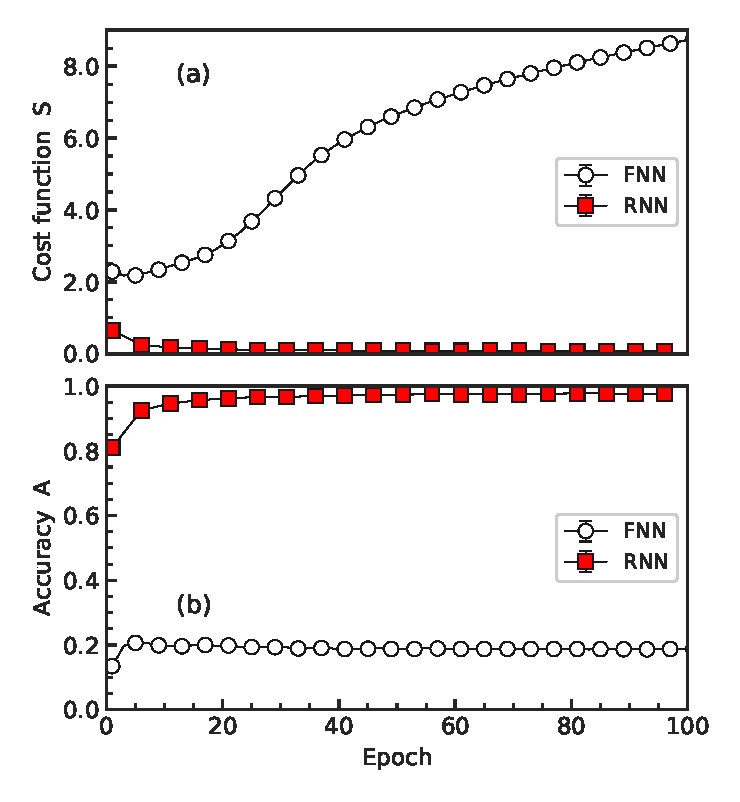
\includegraphics[width=\columnwidth]{./figs/FIG5.eps}
	\caption{
		Demonstration of the importance of pixel ordering for MNIST recognition when FNN is used (circles) and the automatic pixel-position and feature correlation for MNIST recognition when RNN is used (squares). When the pixel ordering [green arrows in Fig. \ref{FIG1}(a)] is scrambled, an FNN cannot be trained adequately to recognize the MNIST images, shown by the rising cost and low accuracy on test data, even
		when the position-feature data are used together in the input to Fig. \ref{FIG2}(a). On the other hand, when the same data are used with an RNN [Fig. \ref{FIG2}(b)] the network can successfully identify the 10 different digits, as shown by the minimal cost entropy and near-perfect test set accuracy.}
	\label{MNIST}
\end{figure}

The MNIST dataset includes $6\times 10^4$ training images and $10^4$ testing images of handwritten numerical digits. One of the images is shown in Fig.~\ref{FIG1}(a). An industrial standard of machine learning is the correct identification of the 10 numerical digits in the MNIST set. It is well-known that deep FNN is an effective tool for this purpose, reaching accuracies above 99\% \cite{schmidhuber_deep}. The output layer shown in Fig. \ref{FIG2} now has $n=10$ nodes, each characterizing a digit, from $0, 1, 2, ..., 9$.

A typical data set to represent an MNIST image has the data structure $P_{ij}$, where $i=1,...28$ is the row number of the pixels, and $j=1,...28$ the column number, and $P$ the grey scale ``ink'' intensity of the writing. Implicitly, when the data is stored according to the order of $i$ and $j$, spatial location (that is, the pixel position specified by $i$ and $j$) follows this order. The configuration file of a 2D Ising model would have a similar data structure where $P$ has only two values, up and down.

To compare with the off-lattice output data, we rewrite a data point $P_{ij}$ by a line of four numbers $[l, i_l, j_l, P_{ij}]$ where $l
=1,2,\dots,28\times 28$ is a sequential number that labels $i_l$ and $j_l$. This has the same data structure as the configurational record obtained from an off-lattice molecular simulation where a typical line reads $[l, x_l, y_l, \theta_l]$. However, there is one important difference: the MNIST data has a correlation between $l$ and $(i_l, j_l)$ in an orderly fashion, whereas in the off-lattice coordinate record, there is no correlation between $l$ and $x_l, y_l$.

If we decorrelate $l$ from $(i_l, j_l)$ but use $(i_l, j_l, P_{i_lj_l})$ as the input, can an FNN still identify the numerical digits? The decorrelation is done by scrambling the line ordering of  $(i_l, j_l, P_{ij})$ data for each digit image.
As demonstrated by the circles in Figs. \ref{MNIST}(a) and (b), the FNN now {\emph {fails}} to learn the correlation between $i, j$ and $P_{i_lj_l}$.
The FNN network looks for the correlation between features (that is, $i, j$ and $P_{ij}$) and the data ordering. This ordering, of course, is destroyed in scrambling the line ordering. We can also demonstrate that the coarse-graining method mentioned in the text helps to reestablish the position-intensity correlation; the plots are omitted here.

A strong contrast is the use of RNN. The three inputs to LSTM blocks in Fig.\ \ref{FIG2}(b) are now $i$, $j$, $P_{ij}$, in a random order because of the intentional data scrambling.
The cost function $S$ and test set accuracy $A$ are shown in Fig.~\ref{MNIST} by squares. The RNN manages to effectively learn the correlation between $i, j$ and $P_{ij}$ and successfully identifies all 10 numerical digits.

\vfill



\section{PCA}





\begin{figure*}[!t]
	\centering
	\includegraphics[width=\columnwidth]{./figs/pca_scatt_e3defect_01.eps}
	\caption{(a) Observations from the comprehensive dataset along the first two principal components. The concentrations around $w_0 = 4$ correspond to corner samples.
	}
\label{FIG:pca_scatt}
\end{figure*}
		
\begin{figure*}[!t]
	\centering
		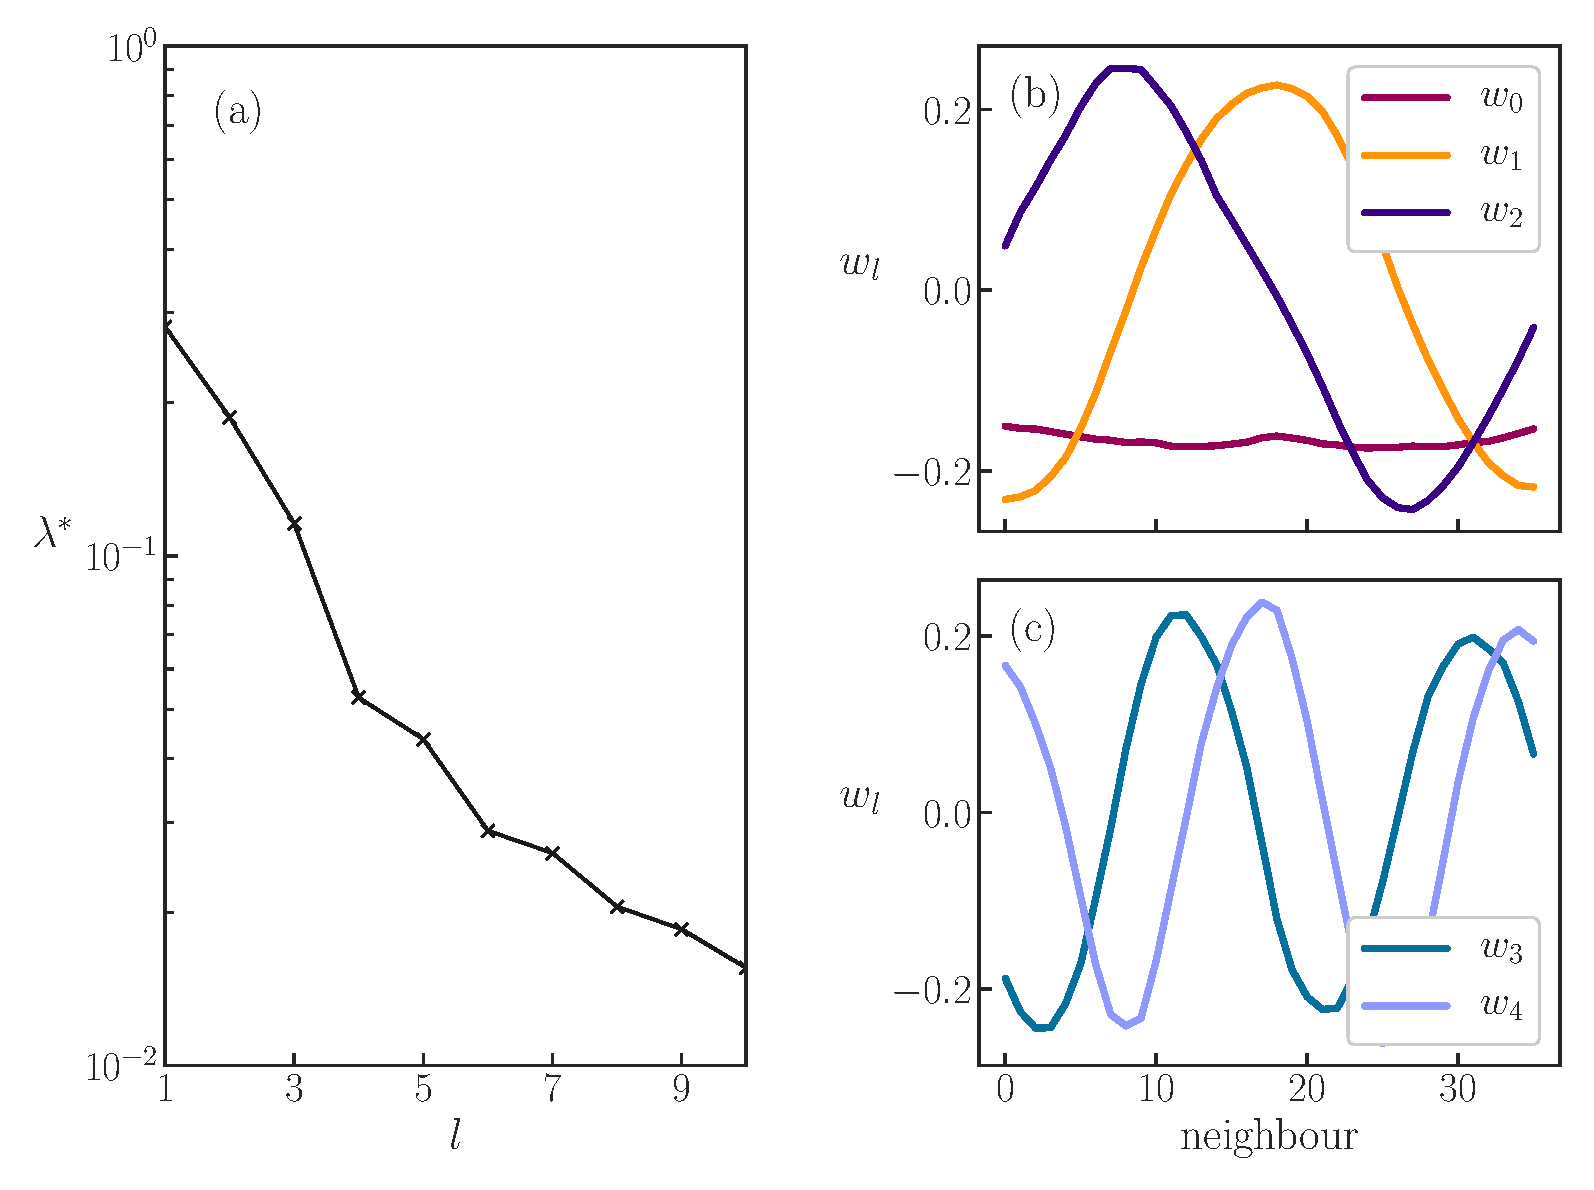
\includegraphics[width=\columnwidth]{./figs/pca_all_e3defect.eps}
	\caption{(a) Explained variance ratios for the normalized comprehensive dataset and (b)-(c) the first five components. See text for discussion.
}
\label{FIG:pca_all}
\end{figure*}

Figure \ref{FIG:pca_all} shows explained variance ratios and the first five componentes of the normalized comprehensive dataset. By inspecting these eigen waveforms we can discern what PCA is looking for. $w_1$ responds to the nematic-isotropic character of neighbours. Since it is nearly a constant form, isotropic feature vectors $\bv{f_I}$ will give $\bv{f_Iw_1} \approx \sum -0.5w_{1i} \approx 5$, and nematic $\bv{f_N}$ will find $\bv{f_Nw_1} \approx \sum 0.6w_{1i} \approx -5$, as is observed in the distribution of Figure \ref{FIG:pca_scatt}. MENTION THE VALUES OF FIGURE 4.4.
The waveforms above $w_1$ have an interesting pattern. They seem to represent higher frequencies of rotation winding around the defect point, and also may be grouped in pairs. Consider the feature vector waveforms in Figures \ref{FIG:prob_samples1} \& \ref{FIG:prob_samples2}. The $1/2$ and $1$ winding number vectors approximate
\begin{align}
f_{1/2}(n_i) &= \sin(2\pi n_i/N_{nn} + \phi)\\
f_{1}(n_i) &= \sin(\pi n_i/N_{nn} + \phi),
\end{align}
for neighbour $n_i$ and random phase $\phi$ since in practice 


\begin{figure*}[!t]
\centering
\begin{minipage}[c]{\columnwidth}
	\centering
	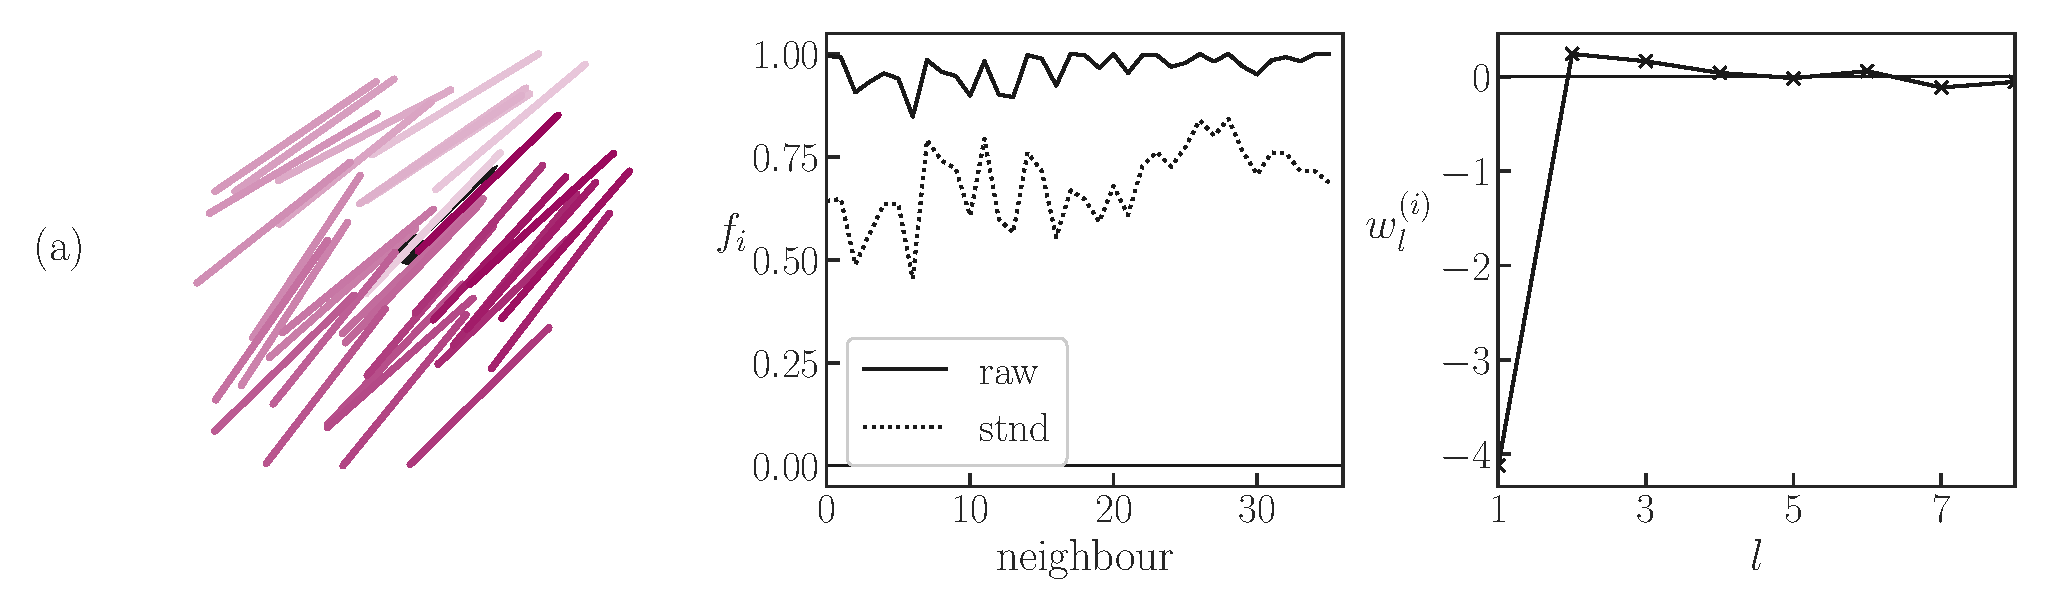
\includegraphics[width=\columnwidth]{./figs/prob_stats_nem.eps}\\
	\vspace{0.5cm}
	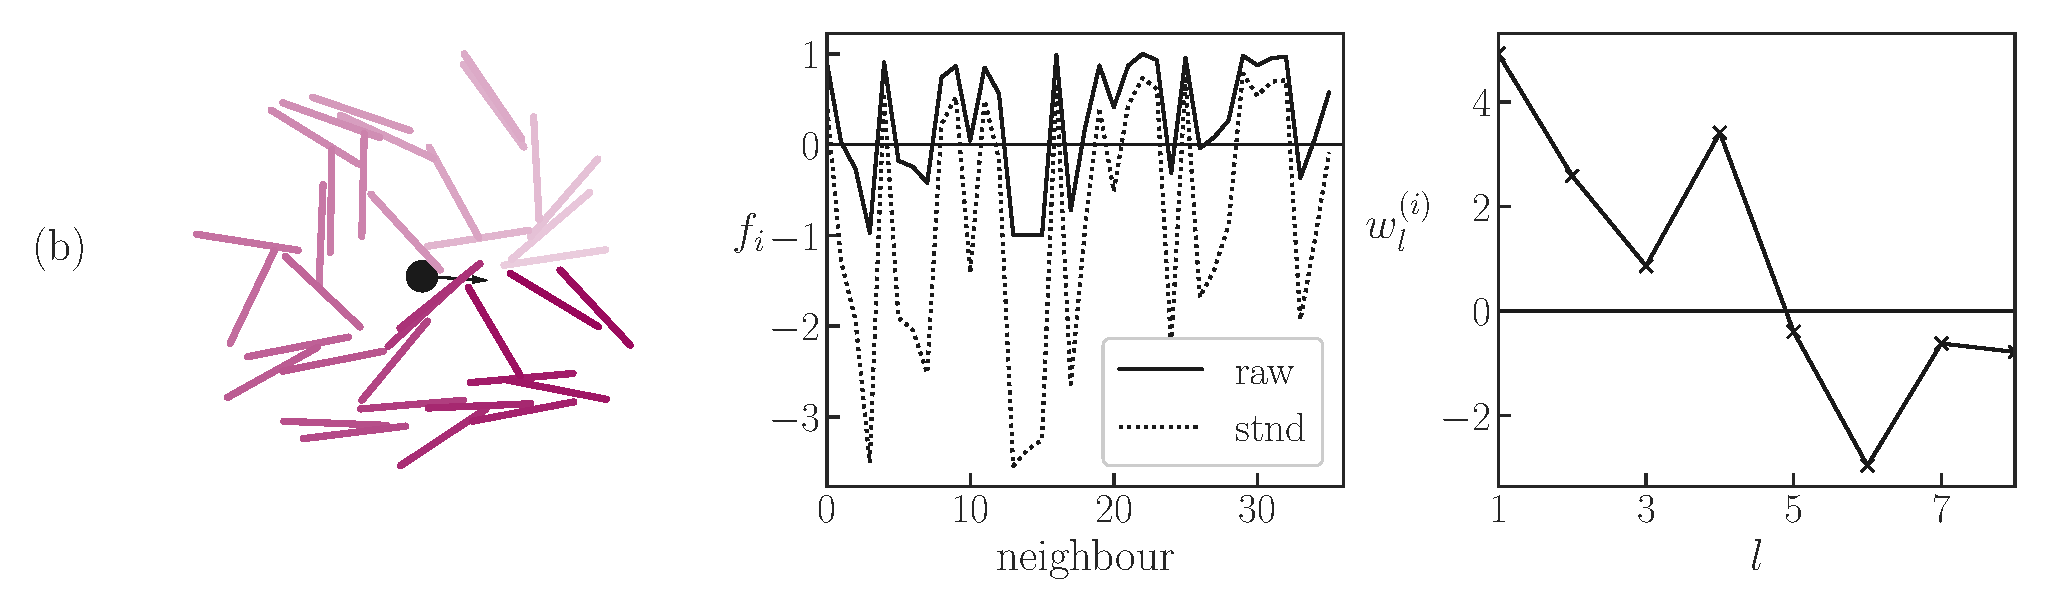
\includegraphics[width=\columnwidth]{./figs/prob_stats_iso.eps}	\end{minipage}%
	\caption{Feature vectors (middle column) and their modified PCA components (right column) for isotropic and nematic neighbours. We can see that $w_1$ captures isotropic and nematic information by the opposing strong responses.
}
\label{FIG:prob_samples3}
\end{figure*}

\begin{figure*}[!t]
\centering
\begin{minipage}[c]{\columnwidth}
	\centering
	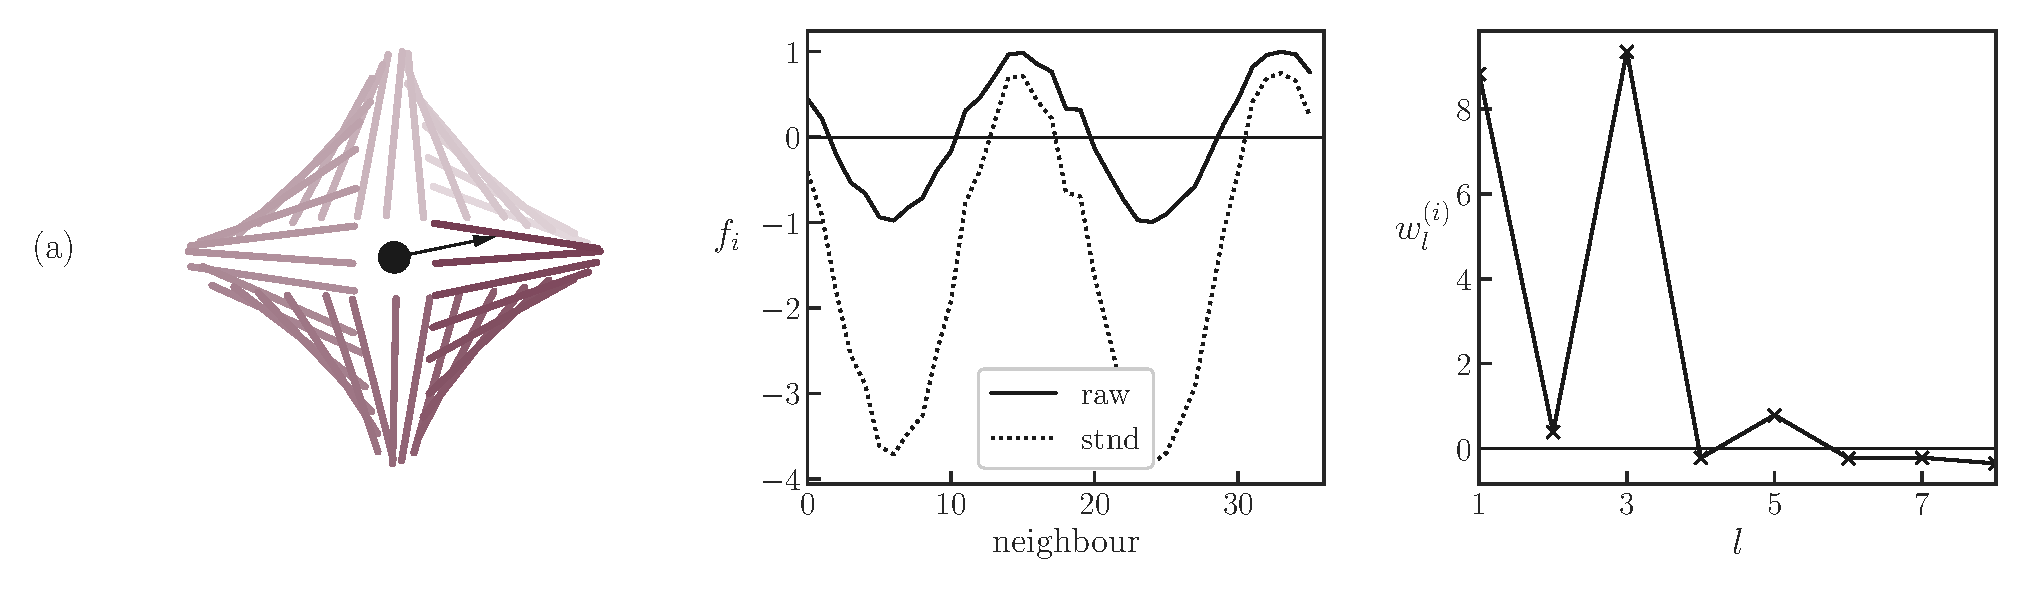
\includegraphics[width=\columnwidth]{./figs/prob_stats_minusone_small_0.eps}\\
	\vspace{0.5cm}
	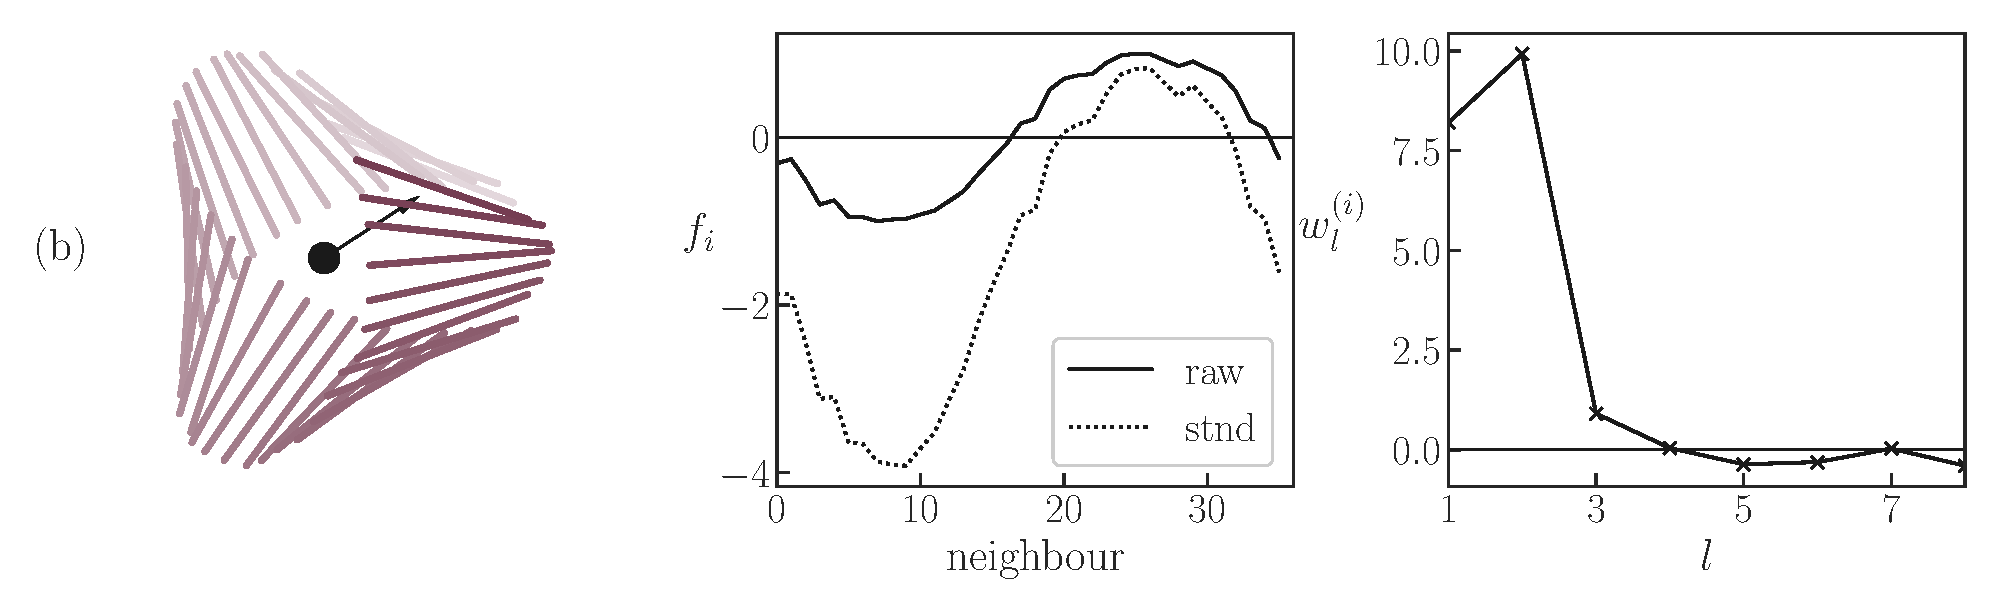
\includegraphics[width=\columnwidth]{./figs/prob_stats_minushalf_small_0.eps}
\end{minipage}%
\caption{Feature vectors (middle column) and their modified PCA components (right column) for $-1$ (a) and $-1/2$ (b) winding numbers. The $-1$ defect shows a high response in the \nth{3} component, with the $-1/2$ defect giving a high response in the \nth{2} component. Both are still highly nematic and give a strong \nth{1} component response.
}
\label{FIG:prob_samples1}
\end{figure*}

\begin{figure*}[!t]
\centering
\begin{minipage}[c]{\columnwidth}
	\centering
	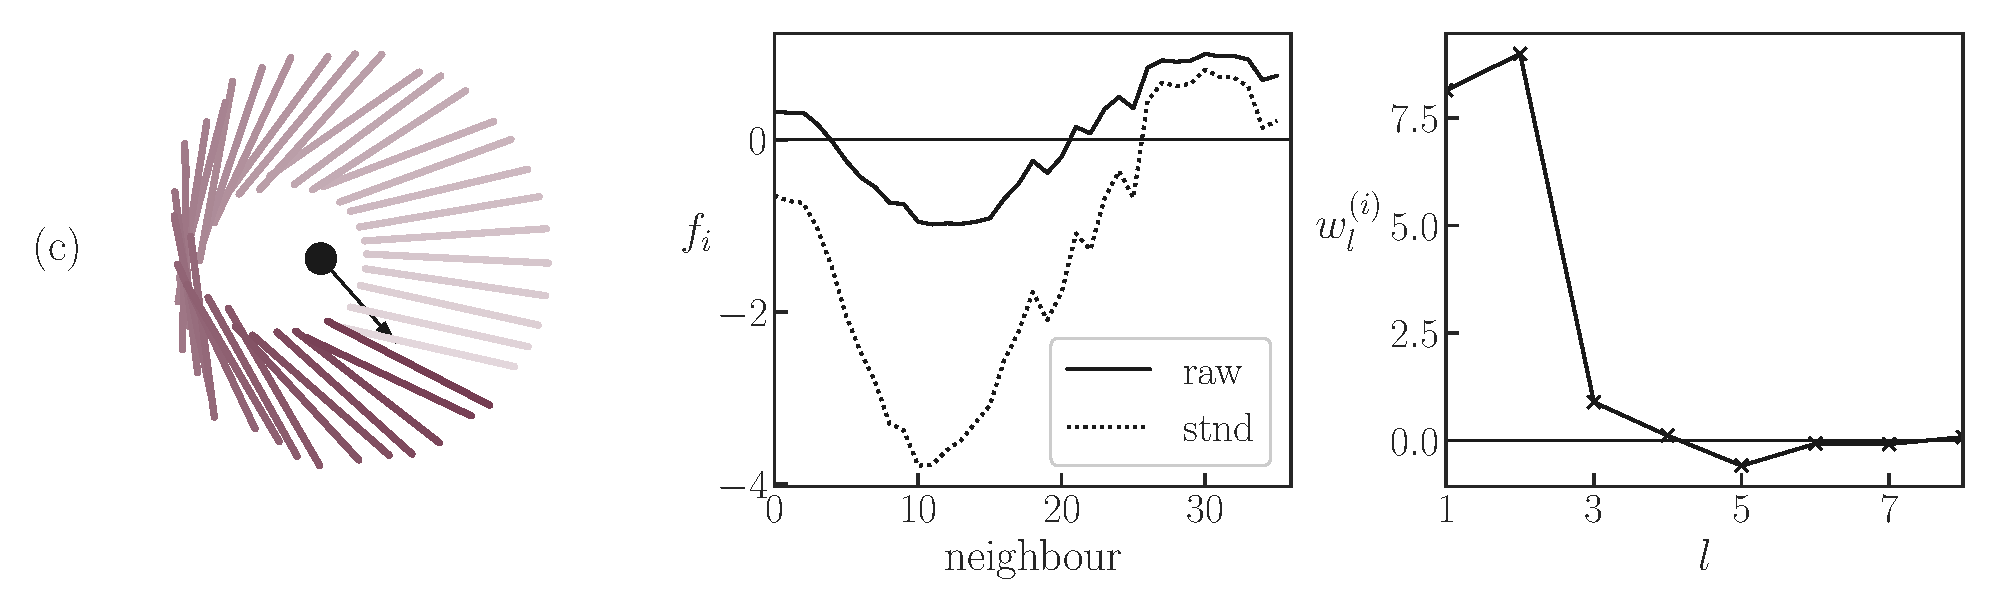
\includegraphics[width=\columnwidth]{./figs/prob_stats_plushalf_small_0.eps}\\
	\vspace{0.5cm}
	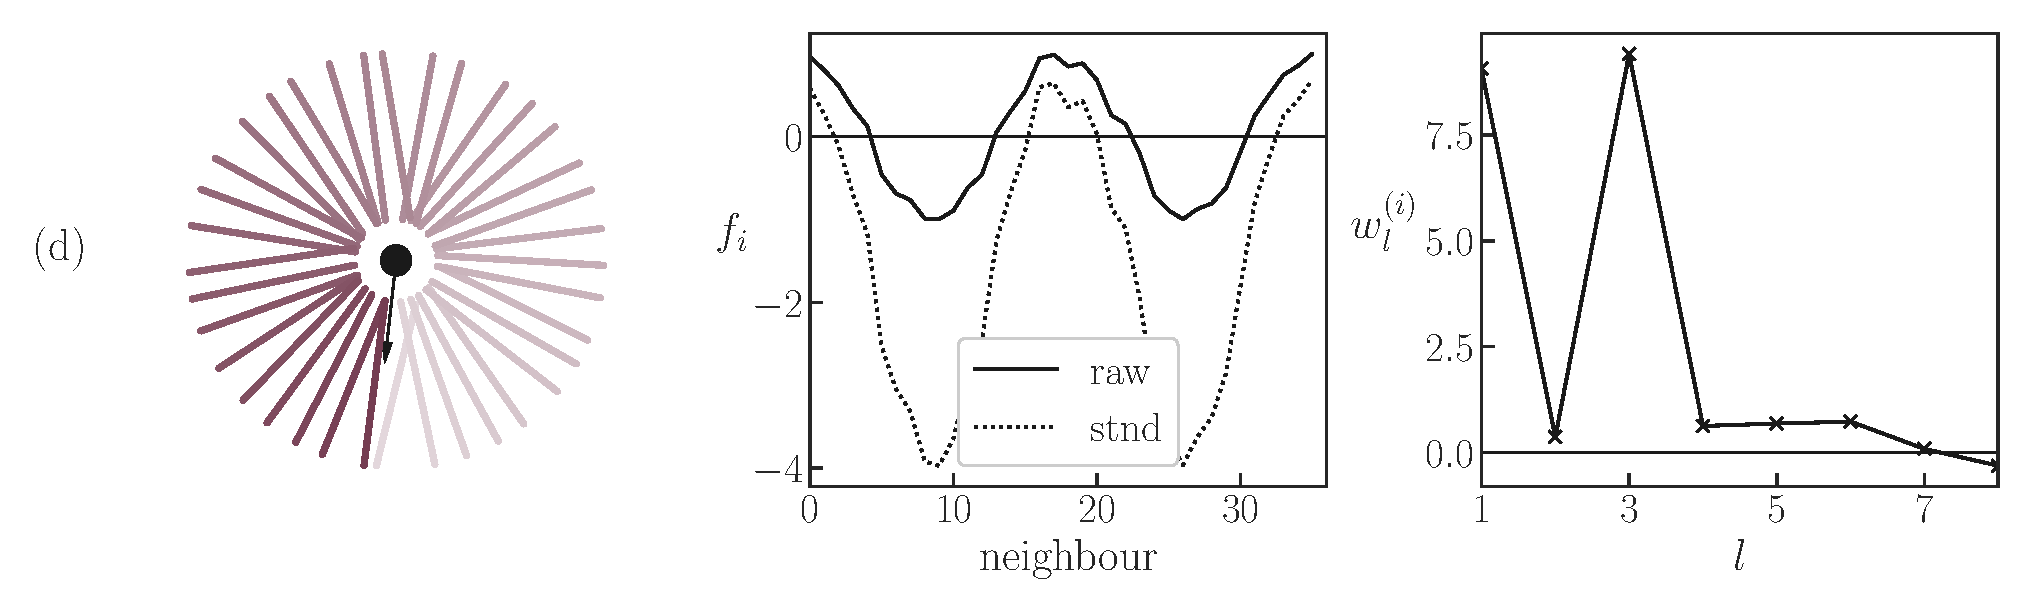
\includegraphics[width=\columnwidth]{./figs/prob_stats_plusone_small_0.eps}
\end{minipage}%
\caption{Feature vectors (middle column) and their modified PCA components (right column) for $+1/2$ (a) and $+1$ (b) winding numbers. The $+1/2$ defect shows a high response in the \nth{2} component, with the $+1$ defect giving a high response in the \nth{3} component. Both are still highly nematic and give a strong \nth{1} component response.
}
\label{FIG:prob_samples2}
\end{figure*}




\textbf{DISCUSS} Go into the topic surrounding the difficulty of avoiding false rotations. This seems to be the main problem with using just th\_jalpha information (polar2) as opposed to our best mode of cos(2*th\_jalpha) (polar). Heat map images show that polar2 can be very sketchy (along w0 at least). File \texttt{edge\_3\_11.47} nblskip 1, px,py = 15,15 and px,py = 15,16 provide two good examples of how different things can be.

Let's map out this discussion on methods.
Three modes to consider: random, winding alignment ``WA'' (polar), winding difference ``WD'' (polar2).
I think we will need a suite of plots here: 
\begin{itemize}
	\item scatter plots of $w_1/w_2$ probably don't need to go to higher comparisons, except it may be interesting on the WA plot
	\item The eigenvalue and vector plots
	\item Probe plots
	\begin{itemize}
		\item smalldefects with all three modes. These could maybe be combined across modes. Otherwise it may feel like relegating to appendix, however random mode colors the rods differently.
		\item iso-nem for WA at least. Does WD capture this? Looks like no. Especially near the phase transition where some skew rods will really throw things off and produce false rotations. It performs fine in nematic regions.
		I just looked at the X-state with WD and 0,1,2, dimensions and it hardly responds to different regions, and also flipflops near the center. false rotations causing issues no doubt.
	\end{itemize}
	\item Many heat map plots
	\begin{itemize}
		\item possibly some of the smalldefects in random mode
		\item run edge\_3\_11.47 showing how WD and WA behave differently
		\item some XTUD images. We should do higher order colouring here. For example, the 3rd vs 2nd dimension colouring should be interesting, though 2nd will colour over 3rd. See note above wrt WD and X-state
		\item Heat maps of smalldefects for WA and WD probably overkill
	\end{itemize}
	\item 
\end{itemize}


\begin{figure*}[!t]
	\centering
	\begin{minipage}[c]{\columnwidth}
		\centering
		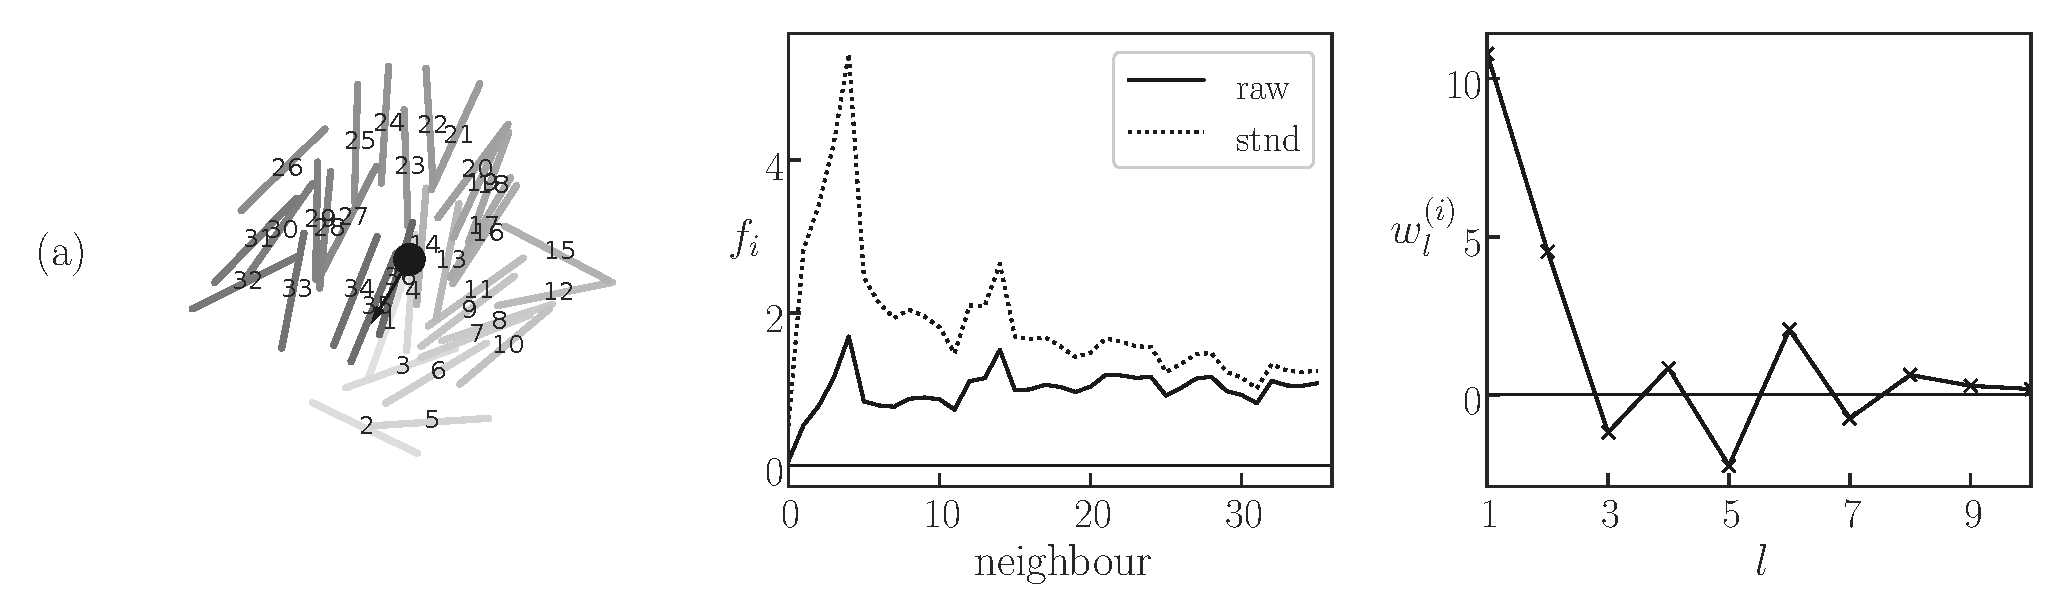
\includegraphics[width=\columnwidth]{./figs/prob_stats_polar2_a.eps}\\
		\vspace{0.5cm}
		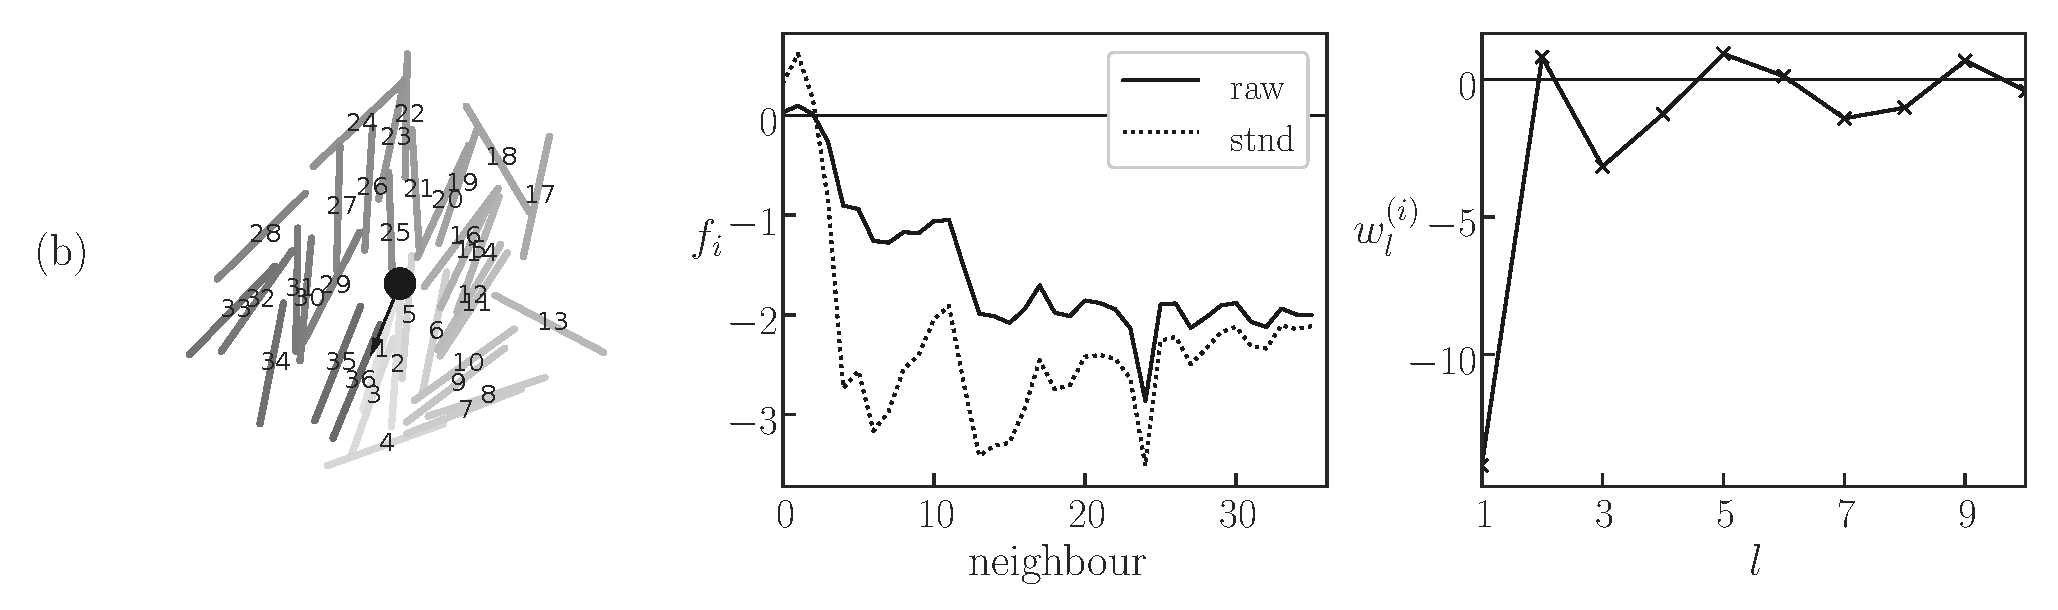
\includegraphics[width=\columnwidth]{./figs/prob_stats_polar2_b.eps}
	\end{minipage}%
	\caption{Feature vectors (middle column) and their modified PCA components (right column) for $+1/2$ (a) and $+1$ (b) winding numbers. The $+1/2$ defect shows a high response in the \nth{2} component, with the $+1$ defect giving a high response in the \nth{3} component. Both are still highly nematic and give a strong \nth{1} component response.
	}
	\label{FIG:prob_polar2}
\end{figure*}









